

\documentclass[8pt, usepdftitle = false]{beamer}
% \imput{../common/beamerthemesimple}
\usetheme{simple}


  \usepackage{xcolor}
  \definecolor{olive}{rgb}{0.3, 0.4, .1}
  \setbeamercolor{itemize/enumerate body}{fg=black}
  \setbeamercolor{title}{fg = green!30!black}
  \setbeamercolor{frametitle}{fg = gray!70!black, bg = white}


% \usepackage{lmodern}
\usepackage[scale = 2]{ccicons}
\usepackage[export]{adjustbox}
\usepackage{amsmath, amsthm, amssymb}
\usepackage{amsfonts}
\usepackage{mathtools}

\usepackage[justification=raggedright,width=\linewidth]{caption}
\usepackage{tikz} 


\usepackage{setspace}

\setbeamertemplate{title page}[default][right,colsep=-4bp,rounded=true,shadow=\beamer@themerounded@shadow]

\setbeamertemplate{caption}[numbered]


%% Options

\setbeamercolor{alerted text}{fg=blue}
\setbeamertemplate{alerted text begin}{\itshape}
\setbeamertemplate{alerted text end}{}

\newenvironment<>{varblock}[2][\textwidth]{%
    \setlength{\textwidth}{#1}
    \begin{actionenv}#3%
        \def\insertblocktitle{\underline{#2}}%
        \par%
        \usebeamertemplate{block begin}}
        {\par%
        \usebeamertemplate{block end}%
    \end{actionenv}}

\setbeamertemplate{blocks}[rounded][shadow=true]
\setbeamercolor{block title}{fg=black,bg=gray!20!white}
\setbeamercolor{block body}{fg=black,bg=gray!10!white}




%% Theorem

% \newtheorem{theorem}{Theorem}

%% Bangla tex


\usepackage{polyglossia}
\setotherlanguage[numerals=Devanagari]{bengali}
\setmainlanguage{english}
\newfontfamily\bengalifont[Script=Bengali]{Akaash}


%% tikx

\usepackage{tikz}
\usetikzlibrary{calc,trees,positioning,arrows,fit,shapes,calc}





\newcommand\blfootnote[1]{%
  \begingroup
  \renewcommand\thefootnote{}\footnote{#1}%
  \addtocounter{footnote}{-1}%
  \endgroup
}



\newcommand\Permute[2][^n]{\prescript{#1\mkern-2.5mu}{}P_{#2}}
\newcommand\Combine[2][^n]{\prescript{#1\mkern-0.5mu}{}C_{#2}}


\renewcommand*{\thefootnote}{\fnsymbol{footnote}}


\usepackage{flexisym}
\usepackage{breqn}

\usepackage[T1]{fontenc}

% \usepackage{mathpazo}
% \renewcommand{\rmdefault}{put}

% \usepackage{fourier} 
% Only use the math font of mathpazo
% \let\temp\rmdefault
% \usepackage{mathpazo}
% \let\rmdefault\temp
% \renewcommand{\rmdefault}{put}


% \usepackage[hyphens]{url}


  % \usefonttheme{professionalfonts} % using non standard fonts for beamer
  % \usefonttheme{serif} % default family is serif

  % \usepackage{gentium}
  \usepackage{multicol}
  \usepackage{mathpazo}



% \renewcommand{\familydefault}{\sfdefault}  


  % color brackets
  \makeatletter
  \newcount\bracketnum
  \newcommand\makecolorlist[1]{%
      \bracketnum0\relax
      \makecolorlist@#1,.%
      \bracketnum0\relax
  }
  \def\makecolorlist@#1,{%
      \advance\bracketnum1\relax
      \expandafter\def\csname bracketcolor\the\bracketnum\endcsname{\color{#1}}%
      \@ifnextchar.{\@gobble}{\makecolorlist@}%
  }
  \let\oldleft\left
  \let\oldright\right
  \def\left#1{%
      \global\advance\bracketnum1\relax 
      \colorlet{temp}{.}%
      \csname bracketcolor\the\bracketnum\endcsname
      \oldleft#1%
      \color{temp}%
  }
  \def\right#1{%
      \colorlet{temp}{.}%
      \csname bracketcolor\the\bracketnum\endcsname
      \oldright#1%
      \global\advance\bracketnum-1\relax
      \color{temp}%
  }
  \makeatother


  \makecolorlist{black,blue,red}






\setbeamertemplate{section in toc}{%
  {\color{firstcolor}\inserttocsectionnumber.}~\inserttocsection}
\setbeamercolor{subsection in toc}{bg=white,fg=black}
\setbeamertemplate{subsection in toc}{%
  \hspace{1.2em}{\color{firstcolor}\rule[0.3ex]{3pt}{3pt}}~\inserttocsubsection\par}


\setbeamerfont{section in toc}{size=\fontsize{6}{8}\selectfont}
\setbeamerfont{subsection in toc}{size=\fontsize{6}{8}\selectfont}
\setbeamerfont{subsection in toc shaded}{size=\fontsize{6}{8}\selectfont}


\makeatletter
\patchcmd{\beamer@sectionintoc}{\vskip1.5em}{\vskip0.5em}{}{}
\makeatother






  \usepackage{twemojis}
  \usepackage{fontspec}
  \usepackage{tikzsymbols}
  \newfontfamily\DejaSans{DejaVu Sans}

% for R
\usepackage[fixed]{fontawesome5}


\setbeamercolor{emph}{fg=red}
\renewcommand<>{\emph}[1]{%
  {\color{purple}\only#2{\rm\itshape}#1}%
}

\setbeamertemplate{frametitle continuation}{}


\usepackage[round,  maxcitenames=10, mincitenames=11]{natbib}
\setlength{\bibhang}{0pt}
\renewcommand{\bibsection}{}
\usepackage{fancybox}


\setbeamertemplate{section page}
{
    \begingroup
    \begin{beamercolorbox}[sep=12pt,center]{section title}
        \usebeamerfont{section title}\insertsection\par
    \end{beamercolorbox}
    \endgroup
}

\setbeamertemplate{subsection page}
{
    \begingroup
    \begin{beamercolorbox}[sep=12pt,center]{section title}
        \usebeamerfont{section title}\insertsection\par
    \end{beamercolorbox}
    \vspace*{-1pt}
    \begin{beamercolorbox}[sep=8pt,center]{subsection title}
        \usebeamerfont{subsection title}\insertsubsection\par
    \end{beamercolorbox}
    \endgroup
}



\newcommand\Var[1]{\mathbb{V}\mathrm{ar}{#1}}



\renewcommand{\emph}[1]{%
{\rm\itshape{\color{purple}#1}}%
}

\renewcommand{\alert}[1]{%
{\rm\itshape{\color{blue}#1}}%
}

\newcounter{mytheorem}
\renewcommand{\themytheorem}{3.\arabic{mytheorem}}
\newcommand{\Thm}[1]{\refstepcounter{mytheorem}\textbf{#1\color{blue}\themytheorem}:}




%================ Give the title ============================##

\title{\LARGE Ch3 - Probability Theory - 2}

\subtitle{{\fontsize{10}{10}\selectfont\color{gray!50!balck} 
(Random Variables and Probability Distributions)} \\
\vspace*{.2cm} Statistics For Business and Economics - I}




\author{Shaikh Tanvir Hossain\vspace*{-.4cm}}
\institute{ East West University, Dhaka\\ Last Updated \today}
\date{\vspace{-5pt}}
% \titlegraphic{\includegraphics[width=300,height=.5\textheight]{Images/EWU.png}}

% \setbeamertemplate{background}{\tikz[overlay,remember picture]\node[opacity=0.90]at (current page){\includegraphics[width=.5\textwidth,left]{EWU.png}};}


\usepackage{hyperref}
\hypersetup{
      pdftitle={Ch3 - Probability Theory - Random Variables and Distributions},
        pdfauthor={Shaikh Tanvir Hossain},
          pdfborder={0 0 0},
       colorlinks,
      citecolor=blue,
      linkcolor=gray!50!black,
    breaklinks=true}





\begin{document}

% input the outline 

\begin{frame}[plain,noframenumbering] 
    \maketitle
\end{frame}
\setbeamertemplate{background}{}
\setlength{\abovedisplayskip}{-2pt}
\setlength{\belowdisplayskip}{4pt}
\setlength{\abovedisplayshortskip}{-3pt}
\setlength{\belowdisplayshortskip}{4pt}


\AtBeginSection[]
{
    \begin{frame}[plain, allowframebreaks]
\setstretch{.1}

        \setlength{\parskip}{1ex}
            \tableofcontents[sections={1-7}, 
            currentsubsection, 
            sectionstyle=show/hide, 
            sectionstyle=show/shaded, 
            ]
    \end{frame}
}


% Hide progress bar and footline on titlepage
\begin{frame}{Outline}
 \vspace*{.2cm}

\begin{center}
\begin{minipage}{10cm}
  \begin{alertblock}{Outline}
  \setstretch{.1}
   \setlength{\parskip}{1ex}
  \tableofcontents[sections={1-10}]
  %   \framebreak
  % \tableofcontents[sections={2}]
\end{alertblock}
\end{minipage}
\end{center}


\end{frame}



\begin{frame}[allowframebreaks]{}

\begin{itemize}
\item In this chapter we start with the second part of the Probability Theory where we will start talking about \emph{random variables} and \emph{probability distributions}. Undoubtedly these two concepts are really the core part of Probability Theory and Statistics. In this chapter we will cover univariate random variables and some univariate probability distributions. These are theoretical distributions which are useful to \alert{model} real life scenarios for one variable only. The next chapter will be about multivariate random variables and joint probability distributions (along with conditional distributions) which is more like an extension of these ideas to multivariate setting.

\item So let's start...\faWalking \faWalking \faWalking.

\end{itemize}

\end{frame}



%---------------------------------------------------------------------------------
\section{Random Variables}
\frame{\sectionpage}

\subsection{Definitions, Discrete and Continuous RVs, and Prob. Distributions}
\frame{\subsectionpage}



\begin{frame}[allowframebreaks]{Random Variables}{Definitions, Discrete and Continuous}

\begin{itemize}

\item What is a random variable? Sometimes we are not interested in the experimental outcomes directly, rather we are interested in some \emph{kind of numerical representation of the experimental outcomes}, the idea of the random variable is essentially this....Here is a rough definition, 


\begin{varblock}{\Thm{Definition } (Random Variables, discrete and continuous)}

A Random Variable is a numerical representation of the outcomes of any random experiment. We often use uppercase or capital letters, for example $X$, $Y$, or $Z$, to denote random variables. 

\end{varblock}

Here are some examples.

\item \textbf{Example 1: Experiment - Tossing a single coin }

\medskip
\alert{Sample Space:} $\Omega = \{H, T\}$

\medskip
\alert{Random Variable:} $X = 1$ for Head and $X = 0$ for Tail. 

\medskip

\item \textbf{Example 2: Experiment - Tossing two coins }

\medskip
\alert{Sample Space:}  $	\Omega = \{(H, H), (H, T), (T, H), (T, T)\}$


\medskip
\alert{Random Variable:} Here it is possible to think about different random variables, for example we can think about \emph{ $X$ is a random variable that counts the number of heads}, then in this case 

\begin{align*}
\text{ when we have outcome } (H, H), \text{ then } X = 2, \\
\text{ when we have outcome } (H, T), \text{ then } X = 1, \\ 
\text{ when we have outcome } (T, H), \text{ then } X = 1, \\ 
\text{ when we have outcome } (T, T), \text{ then } X = 0. 
\end{align*}


\medskip
So here the random variable $X$ takes values $0, 1, 2$. 
\medskip

Note we can also think about different random variables in this setting, for example we can think about \emph{total number of tails}, or \emph{whether we have at least one head}, etc. 

\medskip



\item \textbf{Example 3: Experiment - Tossing three coins }

\medskip
\alert{Sample Space:}  {\small $\Omega = \{{(H, H, H)}, {(H,H,T)}, {(H,T,H)}, {(T,H,H)}, {(T,T,H)}, {(T,H,T)}, {(H,T,T)}, {(T,T,T)} \}	$ }


\medskip
\alert{Random Variable:} here again we can think \emph{ $X$ is a random variable that counts the number of heads}, then in this case 

\begin{align*}
\text{ when we have outcome } {(H, H, H)}, \text{ then } X = 3, \\
\text{ when we have outcome } {(H,H,T)}, \text{ then } X = 2, \\ 
\text{ when we have outcome } {(H,T,H)}, \text{ then } X = 2, \\ 
\text{ when we have outcome } {(T,H,H)}, \text{ then } X = 2, \\ 
\text{ when we have outcome } {(T,T,H)}, \text{ then } X = 1, \\ 
\text{ when we have outcome } {(T,H,T)}, \text{ then } X = 1, \\ 
\text{ when we have outcome } {(H,T,T)}, \text{ then } X = 1, \\ 
\text{ when we have outcome } {(T,T,T)}, \text{ then } X = 0. 
\end{align*}


\medskip
So here the random variable $X$ takes values $0, 1, 2, 3$. 

\framebreak

\item You get the idea of the random variable, actually mathematically a random variable is a function, that takes inputs from the sample space $\Omega$ and gives outputs to the real line $\mathbb{R}$. For example in the experiment where we are tossing three coins, we can think a function $X(\omega)$ where the input $\omega$ is coming from the sample space $\Omega$, and the output will be \emph{total number of heads}, which is going to be a real number in the set $\mathbb{R}$.


\begin{figure}
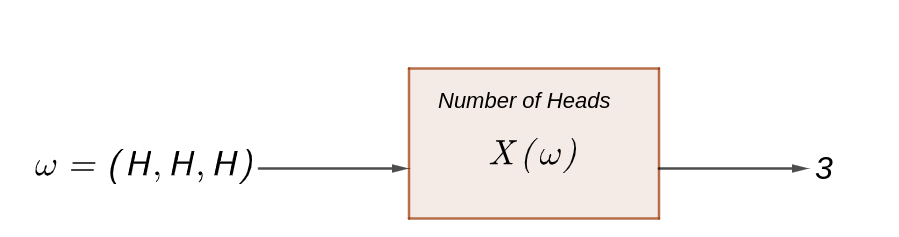
\includegraphics[scale = .3]{Images/Function_1.png}
\end{figure}

\item Like the above picture for any input $\omega$, you can get an output $X(\omega)$, which is going to be a number in $\mathbb{R}$. When we write the random variable $X$, we don't write the input $\omega$.  

\item So again the random variable is actually a function from the sample space $\Omega$ to the real line $\mathbb{R}$. ..... 


\framebreak


\textbf{Discrete and Continuous Random Variables:}


\item[] Depending upon whether the set of values of a random variable is a \emph{countable set} (it could be finite or infinite), or an \emph{uncountable set (which is always infinite)} we can classify the random variables in two types / categories ... 

\medskip
\begin{itemize}
	\item \alert{Discrete Random Variable}: When the random variable takes values in a countable set for example $\{0, 1, 2, 3\}$, or even infinitely countable set like  $\{0, 1, 2, 3, \ldots\}$, we call it a \emph{discrete random variable}. 
	
	\medskip
	\item \alert{Continuous Random Variable}: When the random variable takes values in an uncountable or infinite set, for example $[0, 1]$ or $[0, 30]$ or even $(-\infty, \infty)$, we call it a \emph{continuous random variable}. 


\end{itemize}


\framebreak

\item You might be wondering why we call this \emph{``random''} variable? Any guess? This is because before performing the experiment, the \alert{input of the function is random}. So the \alert{output of the function is also random}. Following picture is useful,


\framebreak

\begin{figure}
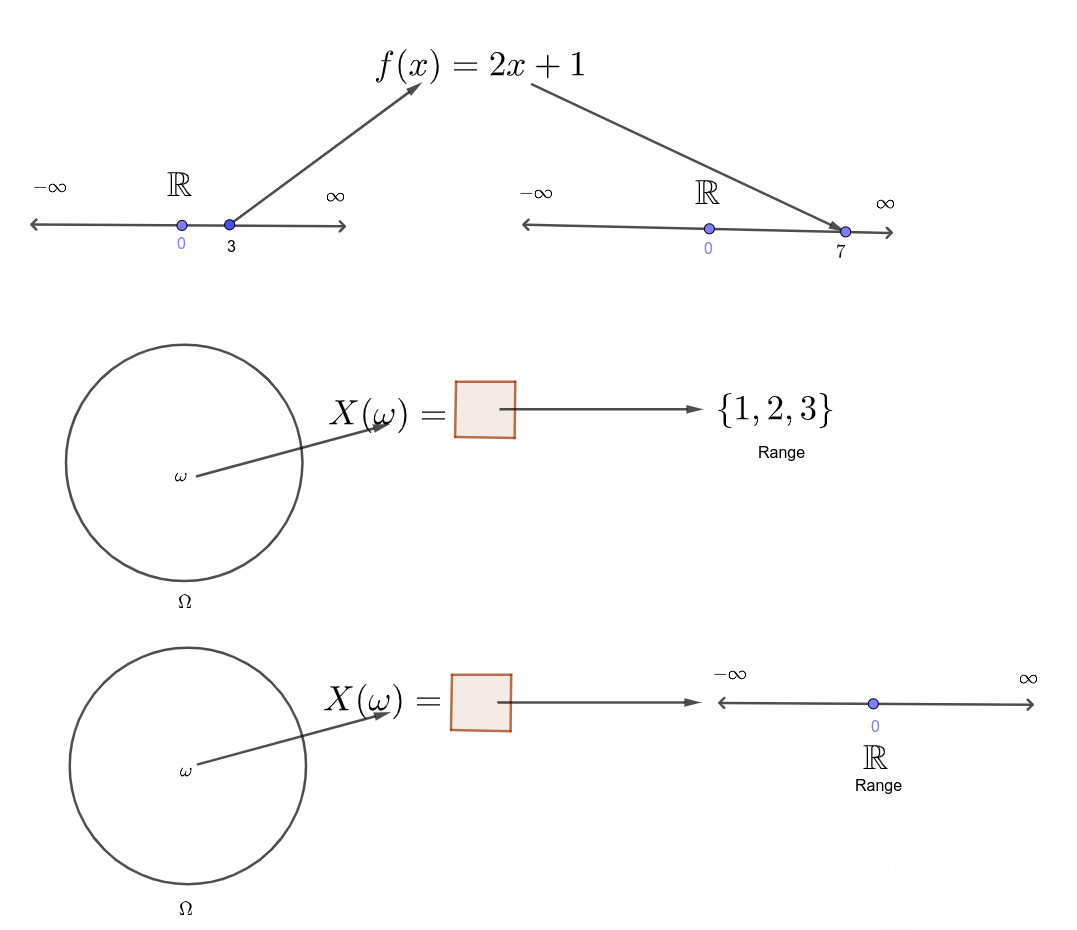
\includegraphics[scale = .2]{Images/RVs_OFs.png}
\caption{From the top, the first one is a mathematical function where the input is not random and the output is also not random (we often call this \alert{deterministic function}). The second one is a \emph{discrete random variable} where the output set is $\{1, 2, 3 \}$. And the third one is a \emph{continuous random variable} where the output set is whole $\mathbb{R}$. Note that for the random variables there is a blank box, this means before performing the experiment we don't know the output, since the input is random, so does the output...}
\end{figure}


\framebreak



\item Let's see some real life examples of random variables. It's important that in many cases the random variable and the values are clear but the sample space is probably not clear. So when we start thinking about random variables, we don't actually think about the actual sample space, rather we think about the random variable and the values it can take. 


\item Following are some examples of discrete random variable  (some examples are taken from \citet*{anderson_statistics_2020}).



\small{
\begin{table}[H]
\begin{tabular}{l|l|l} 
\emph{Random Experiment} & \emph{RV - $X$} & \emph{Possible Values, $x$ } \\ \hline
Toss a coin & 1 - head, 0 - tail & $1, 0$  \\
Roll a die & \# dots in upper face & $1,2,3,4,5,6$ \\
Contact a single customers & 1 - receives, 0 - ignores & $1,0$ \\
Contact $5$ customers & \# customers who receives & $0,1,2,4,5$ \\
Operate a hospital for a day & \# patients who arrive & $0,1,2,3, \ldots$ \\
Offer a customer the choice of  products & product chosen by customer & 
0 - None, 1 - A, 2 - B \\
Randomly pick $10$ EWU students & their occupation status & 1 - job, 0 - no job
\end{tabular} 
\caption{Examples of Discrete Random Variables}		
\end{table}
}

\small{
\raggedright
\begin{table}[H]
\begin{tabular}{l|l|l} 
\emph{Random Experiment} & \emph{RV - $X$} & \emph{Possible Values, $x$ } \\ \hline
Customer visits a web page & time customer spends (in min) & $[0, \infty)$ \\
Taking a bus to Uni & time you have to wait (in min) & $[0, \infty)$ \\
Randomly pick $10$ EWU students & each of their heights (in cm) & $[120, 210]$ \\
A flight from Dhaka to Chittagong & time need to travel (in min) & $[60, 90]$ \\

\end{tabular}
\caption{Examples of Continuous Random Variables}		
\end{table}
}


\end{itemize}
\end{frame}




% \subsection{Calculating Probabilities and Distributions}
% \frame{\subsectionpage}


\begin{frame}[allowframebreaks]{Random Variables}{Calculating Probabilities and Distributions}

\begin{itemize}

\item Our next question is \emph{how do we calculate probabilities for these random variables}, for example, if the \alert{random experiment is tossing two coins} and $X$ is a random variable that counts \alert{the number of heads}, then we know $X$ can take three values $0, 1$ and $2$. Question is how do we calculate $\mathbb{P}(X = 0)$ or $\mathbb{P}(X = 1)$ or $\mathbb{P}(X = 2)$?

\item In this case, we can actually go back to the events associated with it and then calculate the probability of that event using classical definition, for example 

\begin{align*}
	 X &= 0 \text{ is associated with the event } \{ (T, T)\} \\
 	 X &= 1 \text{ is associated with the event } \{ (H,T), (T,H)\} \\
	 X &= 2 \text{ is associated with the event } \{ (H,H)\} \\
\end{align*}

\item Then using the classical definition we can calculate the probabilities, for example 

\begin{align*}
	\mathbb{P}\left(\{ (H,T), (T,H)\}\right) = \frac{2}{4}=\frac{1}{2}
\end{align*} 

\item Doing similarly we get

\begin{align*}
\begin{array}{cccc}
\hline \\
\text{Probabilities of Events:} & \mathbb{P}\left(\{  (T, T) \} \right)  & \mathbb{P}\left(\{ (H,T), (T,H)\}\right) & \mathbb{P}\left(\{ (H,H)\}\right) \\
\hline \\
 \text{Probabilities:} & 1/4 & 1/2 & 1/4 \\
\\
\hline
\end{array}
\end{align*}

Now we can map the same probabilities with the random variables since they are connected with the events, so this gives us, 


\begin{align*}
\begin{array}{cccc}
\hline \\
\text{Probabilities of the Values of } X: & \mathbb{P}(X=0)  & \mathbb{P}(X=1) & \mathbb{P}(X=2) \\
\hline \\
 \text{Probabilities :} & 1/4 & 1/2 & 1/4 \\
\\
\hline
\end{array}
\end{align*}


\item Here $ \mathbb{P}(X=x)$ means, \emph{probability of $X$ taking values $x$}, where $x$ can be $0$, $1$, and $2$. Note that we will write the random variables with uppercase letters and the values with lowercase letters. 


\framebreak

\item Here is another example, when we have tossed three coins, here the sample space is 


{\small $\Omega = \{{(H, H, H)}, {(H,H,T)}, {(H,T,H)}, {(T,H,H)}, {(T,T,H)}, {(T,H,T)}, {(H,T,T)}, {(T,T,T)} \}	$ }

Now we can think about a random variable $X$ that counts the number of heads, then in this case 

\begin{align*}
	 X &= 0 \text{ is associated with the event } \{ (T, T, T)\} \\
 	 X &= 1 \text{ is associated with the event } \{ (H,T,T), (T,H,T), (T,T,H)\} \\
	 X &= 2 \text{ is associated with the event } \{ (H,H,T), (H,T,H), (T,H,H)\} \\
	 X &= 3 \text{ is associated with the event } \{ (H,H,H)\}\\
\end{align*}


\framebreak

\item With the same idea in this case we can calculate,

{\scriptsize
\begin{align*}
\begin{array}{ccccc}
\hline \\
\text{Probabilities of Events:} & \mathbb{P}\left(\{ (T,T,T) \} \right)  & \mathbb{P}\left(\{ (H,T,T), (T,H,T), (T,T,H)\}\right) & \mathbb{P}\left(\{ (H,H,T), (H,T,H), (T,H,H)\}\right) & \mathbb{P}\left(\{ (H,H,H)\}\right) \\
\hline \\
 \text{Probabilities:} & 1/8 & 3/8 & 3/8 & 1/8 \\
\\
\hline
\end{array}
\end{align*}
}

\item Now we can map the same probabilities with the random variables since they are connected with the events, for example 

\begin{align*}
\begin{array}{ccccc}
\hline \\
\text{Probabilities of the Values of } X:& \mathbb{P}(X=0)  & \mathbb{P}(X=1) & \mathbb{P}(X=2) & \mathbb{P}(X=3) \\
\hline \\
 \text{Probabilities:} & 1/8 & 3/8 & 3/8 & 1/8 \\
\\
\hline
\end{array}
\end{align*}


\item Here again $ \mathbb{P}(X=x)$ means, probability of $X$ taking values $x$, where $x$ can be $0$, $1$, $2$ and $3$. 





% \begin{itemize}
% 	\item $\mathbb{P}(\{0\}) = \mathbb{P}(X = 0)$ or probability that the random variable will take value $0$ and 
% 	\item $\mathbb{P}(\{1\}) = \mathbb{P}(X = 1)$ or probability that the random variable will take value $1$ and
% 	\item $\mathbb{P}(\{2\}) = \mathbb{P}(X = 2)$ or probability that the random variable will take value $2$ and 
% 	\item $\mathbb{P}(\{3\}) = \mathbb{P}(X = 3)$ or probability that the random variable will take value $3$,
% \end{itemize}




\framebreak


\item Interestingly with this information we can also calculate probabilities when our random variable $X$ takes values in different kinds of intervals (recall the open and closed intervals we saw before, like $[2, 3]$ and $(2, 3]$, etc) 

\item For example we can calculate 




\begin{align*}
	&\mathbb{P}(X \in [1, 1.5)) \\
	&\mathbb{P}(X \in [4, 10000)) \\
	&\mathbb{P}( X \in [1, 2)) \\
\end{align*}





\item The idea is pretty simple, we will \emph{use the probabilities where $X$ actually takes its values}, for example, if we have 



\begin{align*}
\begin{array}{cccc}
\hline \\
& \mathbb{P}(X=0)  & \mathbb{P}(X=1) & \mathbb{P}(X=2) \\
\hline \\
 \text{Probabilities} & 1/4 & 1/2 & 1/4 \\
\\
\hline
\end{array}
\end{align*}


then we can calculate 

\begin{align*}
& \mathbb{P}(X \in[1,2])  = \mathbb{P}(X=1) + \mathbb{P}(X=2) = 1/2 + 1/4 = 3/4 \\
& \mathbb{P}(X \in[2,3]) = \mathbb{P}(X=2)  = 1/4 \\
& \mathbb{P}(X \in[0,2]) = \mathbb{P}(X=0) + \mathbb{P}(X=1) + \mathbb{P}(X=2) = 1/4 + 1/2 + 1/4 = 1 \\
\end{align*}



% \item This is because, 


% \begin{align*}
% \begin{array}{ccccc}
% \hline \omega &  {(H,H,H)} &  {(H,H,T)} &  {(H,T,H)} &  {(T,H,H)} \\
% \hline X(\omega) & 3 & 2 & 2 & 2 \\
% \hline \\
% \hline \omega &    {(T,T,H)} &  {(T,H,T)} &  {(H,T,T)} &  {(T,T,T)} \\
% \hline X(\omega)  & 1 & 1 & 1 & 0 \\
% \hline
% \end{array}
% \end{align*}

 
%  \item Now we can calculate $\mathbb{P}(\{ (H,T,T), (T,H,T), (T,T,H)\})$, and then that will be $\mathbb{P}(X =1)$.

\framebreak

\item You can try to calculate ... 


\begin{align*}
	&\mathbb{P}(X \in [1, 1.5)) \\
	&\mathbb{P}(X \in [4, 10000)) \\
	&\mathbb{P}( X \in [1, 2)) \\
\end{align*}







% \item There is a very important point of thinking about random variables, that is


% \vspace*{.2cm}
% \emph{Once we start thinking about random variables, now we have a \alert{new sample space $\mathbb{R}$}, then we can think about \alert{different events in the new sample space $\mathbb{R}$}, and forget about the original sample space $\Omega$}
% \vspace*{.2cm}


% \item Since now we have a new sample space $\mathbb{R}$, we can think about different events in $\mathbb{R}$ (which are subsets of $\mathbb{R}$) and then maybe we can calculate probability in these events, for example 





\item for the probabilities we wrote above, we can write them slightly differently, for example 



\begin{align*}
	&\mathbb{P}(X \in [1, 1.5)) \text{ or we write } \mathbb{P}( 1 \leq X <  1.5)\\
	&\mathbb{P}(X \in [4, 10000)) \text{ or we write } \mathbb{P}( 4 \leq X <  10000)\\
	&\mathbb{P}(X \in [1, 2)) \text{ or we write } \mathbb{P}( 1 \leq X <  2)\\
\end{align*}


\framebreak



\item Finally always remember since $\mathbb{R}$ includes everything or all the possible values of all kinds of random variables, we will always have $\mathbb{P}(\mathbb{R}) = 1$ or $\mathbb{P}(X \in (-\infty, \infty)) = 1$


\item \alert{CAVEAT \faMugHot :} It turns out that it is not easy to calculate probabilities in $\mathbb{R}$, and there might be some issues, there are some bad sets / intervals where we cannot calculate probabilities with a consistent way. To explain it fully we need to talk about measurability issues, which is beyond the scope of this course, so we will simply assume that it is possible to calculate probabilities in the interval of $\mathbb{R}$, and you can ignore this comment if you want!


\framebreak

\item \textbf{Probability Distributions of a Random Variable}

\item The last topic for this part is talking about \emph{probability distribution of a random variable}. Here is an informal definition, 


\begin{varblock}{Probability Distribution of a Random Variable}
	If $X$ is a random variable then the probability distribution of $X$ is the collection of \emph{all probabilities} of different possible intervals in $\mathbb{R}$, for example $\mathbb{P}(X \in [2, 3])$ or $\mathbb{P}(X \in [1, 5])$, etc. If $X$ is a \alert{discrete random variable} then the probability distribution means \emph{how the probabilities are distributed on the values of $X$}, since these probabilities are enough to calculate the probabilities of different intervals in $\mathbb{R}$ for $X$.
\end{varblock}


\item So when $X$ is a continuous random variable the idea of probability distribution is a bit different, we will see that later, but when $X$ is a discrete random variable, the probability distribution means all the probabilities of the form $\mathbb{P}(X = x)$ for all possible values $x$ that $X$ can take. For example, here is a probability distribution a random variable that we already saw



\begin{align*}
\begin{array}{cccc}
\hline \\
& \mathbb{P}(X=0)  & \mathbb{P}(X=1) & \mathbb{P}(X=2) \\
\hline \\
 \text{Probabilities} & 1/4 & 1/2 & 1/4 \\
\\
\hline
\end{array}
\end{align*}




% \item \emph{The probability distribution of a random variable $X$ is the collection of all probabilities of the form $\mathbb{P}(X \in C)$ for all sets $C$ of real numbers such that $\{X \in C\}$ is an event.}



% \item Here for a random variable $X$, the probability distribution means how the probabilities are distributed on the real line $\mathbb{R}$.

% \begin{varblock}{Distribution of a random variable}
% 	Let $X$ be a random variable. The distribution of $X$ is the collection of all probabilities of the form $\mathbb{P}(X \in C)$ for all sets $C$ of real numbers such that $\{X \in C\}$ is an event.
% \end{varblock}



\framebreak


\item Do you think we always have to find probabilities by going back to original sample space? The answer is NO. There are actually two nice functions on the real line $\mathbb{R}$, which helps to calculate probabilities when the random $X$ takes values in different kinds of intervals.

\item For discrete random variable this function is known as \alert{probability mass function} or in short \alert{PMF}. The idea of this function is same as the probability distribution we just talked about, but here we will have a function that gives us the probabilities of the form $\mathbb{P}(X = x)$ for all possible values $x$ that $X$ can take. 

\item and for continuous random variable this function is known as \alert{probability density function} or in short \alert{PDF}.

\item Next we will start talking about discrete and continuous random variables and their distributions. 





\end{itemize}
\end{frame}



\section{Discrete Random Variables}
\frame{\sectionpage}

\subsection{1. Probability Distribution and the idea of PMF}
\frame{\subsectionpage}




\begin{frame}[allowframebreaks]{Probability Distributions}{Idea of PMF}

\begin{itemize}

\item The distribution of a discrete random variable is known as \emph{discrete probability distribution}. We already saw examples of probability distribution of a discrete random variable. And we know that for a discrete random variable it is  always enough to know the \emph{probabilities at all values $x$} that the discrete random variable can take. This means we need to know $\mathbb{P}(X = x)$ at all $x$ in the range of $X$.


\item Again here is another example of a discrete probability distribution when $X$ is a random variable that counts the number of heads when we toss three coins. We can write the probability distribution of this random variable as follows,



\begin{align}\label{pmf_1}
\mathbb{P}(X=x)= \begin{cases} 1/8 & \text { when } x = 0 \\ 
3/8 & \text { when } x = 1 \\ 
3/8 & \text { when } x = 2 \\ 
1/8 & \text { when } x = 3 \\ 
0 & \text {for any other numbers in } \mathbb{R}\end{cases}
\end{align}



\framebreak

\item The idea of \emph{Probability mass function or PMF} is just a function of $x$ which gives us $\mathbb{P}(X = x)$ directly, it's like if you know the PMF of a discrete random variable, you know the distribution of the random variable. Here is the formal definition of PMF,

\begin{varblock}{\Thm{Definition } (Probability Mass Function (PMF))}
If $X$ is a discrete random variable then the probability mass function (in short PMF) of $X$, denoted by $f$, is defined as the function such that \alert{for all $x \in \mathbb{R}$},

$$
f(x)=\mathbb{P}(X=x)
$$

The set $\{x: f(x)>0\}$ is called the \alert{support of (the distribution of) $X$}.
\end{varblock}

\item It's important to note that this function is defined for all real numbers but when it has positive values we call the set of those points \emph{the support of the distribution}. For example the distribution that we saw, we can think about following PMF function, 




\begin{align}\label{pmf_1}
f(x)= \begin{cases} 1/8 & \text { if } x=0 \\ 
3/8 & \text { if } x=1 \\ 
3/8 & \text { if } x=2 \\ 
1/8 & \text { if } x=3 \\ 
0 & \text { otherwise }\end{cases}
\end{align}


\framebreak

\item You will understand the importance of PMF when we start talking about theoretical distributions, but for now you should think \emph{if someone gives you the PMF of a discrete random variable, then you can calculate any probabilities for the random variable can possibly take}.

\framebreak

\item Since it's a function we can actually plot this function, here is a plot 

\begin{figure}
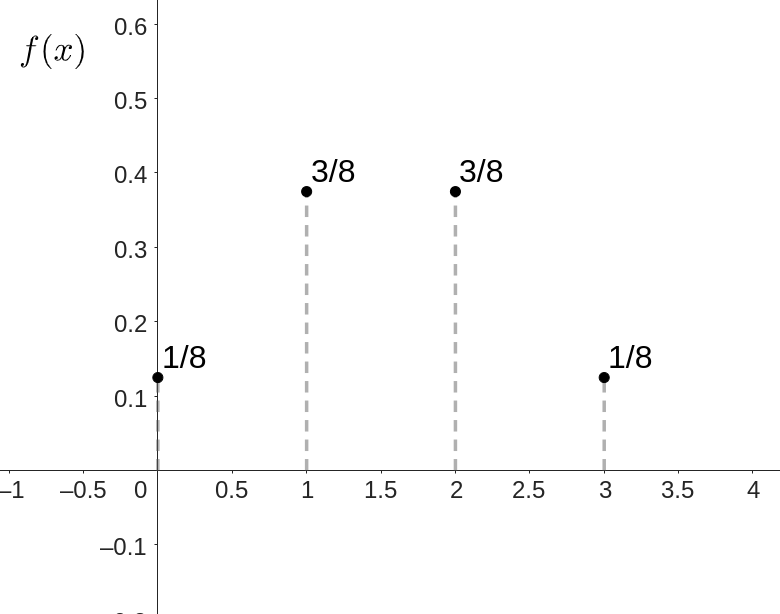
\includegraphics[scale = .3]{Images/pmf_1.png}
\caption{Plot of the PMF in \eqref{pmf_1}} 
\end{figure}

\item The PMF has two important properties, both are easy to understand

\medskip
\begin{varblock}{\Thm{Theorem } (Properties of PMF)}
\begin{itemize}
\item \textbf{The Sum of all PMF Values is 1}: This means if $x_1, x_2, \ldots x_k$ are  all the possible values of a discrete random variable $X$, then 

\begin{align*}
	\sum_{i=1}^{k} f\left(x_i\right)= f(x_1) + f(x_2) + \ldots  f(x_k) = 1
\end{align*}


\item \textbf{The Probability of an Interval in $\mathbb{R}$ can be Calculated as the Sum of PMF Values in the Set}: For example if we are talking about an interval $[2, 3]$, then we can calculate $\mathbb{P}(X \in [2, 3])$ with

$$
\mathbb{P}(X \in [2, 3]) = \mathbb{P}(2 \leq X \leq  3)  \sum_{x_i \in [2, 3]} f\left(x_i\right)
$$
\end{itemize}

\end{varblock}
\medskip

\framebreak


\item The first one is obvious, it says if you sum all the PMF values, then you should get $1$. You already know this since probabilities have to be summed to $1$ for all values when we are talking about discrete random variables. 

\item The second one says the probability of any interval in $\mathbb{R}$ can be calculated by adding the PMF values in that interval. We already saw the application of this rule in page $19/38$. Recall we calculated 

\begin{align*}
\mathbb{P}( X \in [1, 1.5)) = \mathbb{P}(X = 1) = f(1) =  \frac{3}{8}
\end{align*}


\item The key thing to understand here is \emph{knowing PMF is enough to calculate probabilities of different intervals in $\mathbb{R}$}.


\framebreak


\item It is important to mention that \cite{anderson_statistics_2020} uses the terminology \emph{probability function} for PMF. But essentially they are same thing. So if you are reading Chapter 5.2 in \cite{anderson_statistics_2020}, then \alert{probability function} means \alert{probability mass function}. Because probability mass function or PMF is more common in the literature I will use PMF.

\framebreak

\item A question remains, how do we use the idea of PMF in real life examples, actually we will later see that in real life we will model probability using some theoretical distributions, e.g., for discrete random variables we have Discrete Uniform, Bernoulli, Binomial, Poisson, etc. And similarly for continuous random variables we have Uniform, Normal,  Exponential, etc. 

\item For now let's understand the idea of PMF using an empirical data. In this case we can call this \emph{empirical probability mass function}, notice this is very similar to calculating \emph{relative frequency}. However you need to be careful, since this is not the actual probability mass function, since the actual probability mass function can be calculated only using the population. 

\framebreak

\item \Thm{Example } (Random Variable and empirical PMF - Soft Drink example from \cite{anderson_statistics_2020}). Recall the soft drink example we saw before. The data was available for a soft drink company for \emph{last $50$ sales}, here is the data 


\begin{figure}[H]
\centering
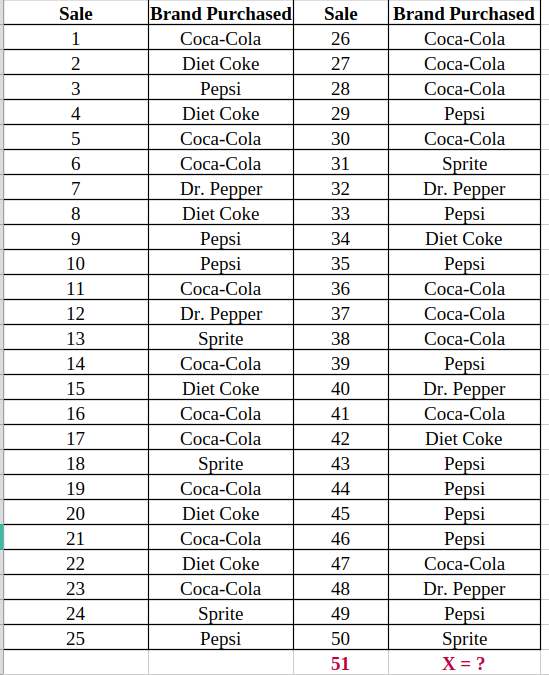
\includegraphics[scale = .3]{Images/softdrink_1.png}	
\caption{Note that 51$st$ sale is a question mark, so we can think about a random variable in that place}
\end{figure}



\framebreak


Here we can think about a random experiment, that is \emph{sales of the $51$st soft drink}, Now we can think about a random variable $X$ that represents soft drink brand. And here is how we can think about a random variable (Keep in mind that a random variable is always a number!)

\medskip
\begin{align*}
X = 1 &\text{ for Coca-Cola} \\
X = 2 &\text{ for Diet Coke} \\
X = 3 &\text{ for Dr. Pepper} \\
X = 4 &\text{ for Pepsi} \\
X = 5 &\text{ for Sprite} \\
\end{align*}



\item Since we already have the frequency distribution, we can write,


    \begin{table}[H]
    \begin{tabular}{c|c|c|c}
      \hline Brand & RV $X$ & Frequency & Relative Frequency and f(x)\\
      \hline Coca-Cola & $X = 1$ & 19 & 0.38 \\
      \hline Diet Coke & $X = 2$ & 8 & 0.16  \\
      \hline Dr. Pepper & $X = 3$ & 5 & 0.1  \\
      \hline Pepsi & $X = 4$ & 13 & 0.26  \\
      \hline Sprite & $X = 5$ & 5 & 0.1  \\
      \hline Grand Total & & 50 & 1  \\
      \hline
\end{tabular}
  \end{table}


\medskip

We can also simply write the \emph{empirical PMF} as

\begin{table}
\centering
\begin{align*}
\begin{array}{c|c}
x & f(x)  \\ \hline
1 & 19/50 = .38 \\
2 & 8/50 = .16 \\
3 & 5/50 = .1 \\
4 & 13/50 = .26 \\
5 & 5/50 = .1 \\
\hline
\end{array}
\end{align*}
\end{table}

\medskip




\item \alert{Again be careful:} We have constructed an \emph{empirical PMF}, and this is not the \emph{true PMF of a random variable $X$ is for the population}, 

\item \emph{Question: What is the population here?}, \alert{Ans:} The data of all sales starting from the opening of the store till it ends the store... so if we can get the population data then we can calculate the \emph{true PMF} of the random variable $X$


\item But in this case is impossible to get the population and calculate the true PMF, so we can only calculate the empirical PMF using a sample, and one can say it's an estimate of the true PMF.

\item Later we will see that for the population we will usually use the idea of theoretical distributions.. .... So we will assume our true PMF follows some \emph{known form of distributions}.... but more on this later...






% , and we can think about a random variable $X$ that counts the brand of the soft drink. So here the possible values of $X$ are $\{Coca-Cola, Diet Coke, Dr. Pepper, Pepsi, Sprite\}$.


% \item \Thm{Example } (Random Variable and PMF - Empirical Example from \cite{anderson_statistics_2020})


% \item Suppose our random variable $X$ is the number of cars sold per day at DiCarlo Motors in Saratoga, New York and we know it can be $0, 1, 2, 3, 4$ or $5$.


% \item Now over the past $300$ days, DiCarlo has experienced - 

% \begin{itemize}
% 	\item $54$ days with no (or $0$) automobiles sold, 
% 	\item $117 $ days with $1$ automobile sold, 
% 	\item $72$ days with $2$ automobiles sold, 
% 	\item $42$ days with $3 $ automobiles sold, 
% 	\item $12$ days with $4$ automobiles sold and 
% 	\item $3$ days with $5$ automobiles sold.
% \end{itemize}


% \item If we think this is our population then with this population we can write following probability mass function.


% \begin{table}
% \centering
% \begin{align*}
% \begin{array}{c|c}
% x & f(x)  \\ \hline
% 0 & 54/300 = .18 \\
% 1 & 117/300 = .39 \\
% 2 & 72/300 = .24 \\
% 3 & 42/300 = .14 \\
% 4 & 12/300 = .04 \\
% 5 & 3/300 = .01
% \end{array}
% \end{align*}
% \end{table}

% \item So the PMF is 

% \begin{align*}
% f(x)= \begin{cases} .18 & \text { if } x=0 \\ 
% .39 & \text { if } x=1 \\ 
% .24 & \text { if } x=2 \\ 
% .14 & \text { if } x=3 \\
% .04 & \text { if } x=4 \\
% .01 & \text { if } x=5 \\
% 0 & \text { otherwise }\end{cases}
% \end{align*}


\end{itemize}
\end{frame}



\subsection{2. CDF, quantiles and percentiles}
\frame{\subsectionpage}

\begin{frame}[allowframebreaks]{Probability Distributions}{CDF for Discrete R.V.}

\begin{itemize}

\item If we know probability distribution of a discrete random variable, we can also calculate \emph{cumulative probabilities}. Cumulative Probability means \emph{probabilities up-to a certain value}. For example, following is a cumulative probability (you already know this!) 

\begin{align*}
	\mathbb{P}(X \leq 2)
\end{align*}

\item For a random variable $X$, this means \alert{the probability of $X$ taking value less than or equal to $2$}. 

\item For example if the distribution and PMF of a random variable is given as, 

\begin{align*}
\mathbb{P}(X = x) = f(x)= \begin{cases} 1/8 & \text { if } x=0 \\ 
3/8 & \text { if } x=1 \\ 
3/8 & \text { if } x=2 \\ 
1/8 & \text { if } x=3 \\ 
0 & \text { otherwise }\end{cases}
\end{align*}

\item Then from this we can calculate,

\begin{align*}
	\mathbb{P}(X \leq 2) &= \mathbb{P}(X = 0) + \mathbb{P}(X =1) + \mathbb{P}(X = 2)
	\\ &= f(0) + f(1) + f(2) \\
	&=1/8 + 3/8 + 3/8 = 7/8
\end{align*}

\framebreak


\item Like PMF represents probabilities in terms of a function. For cumulative probabilities we have a function called \emph{cumulative distribution function} in short CDF. 

\item So CDF simply gives cumulative probabilities. It is a function defined on the real line, where for any value $x$ it gives the cumulative probability upto that value. Here is the formal definition,

\begin{varblock}{\Thm{Definition } (The cumulative distribution function (CDF))}
	The Cumulative Distribution Function or CDF of of a random variable $X$ is the function $F(x)$ defined as 

\begin{align*}
F(x)=\mathbb{P}(X \leq x), \quad \text{ for } -\infty < x < \infty
\end{align*}

\medskip

If $X$ takes values $x_1, x_2, \ldots, x_k$, and $f(x)$ is the PMF, then 

\begin{align*}
F(x) = \sum_{x_i \leq x} f(x_i) 
\end{align*}


\end{varblock}

\framebreak

\item For example, if this is the PMF

\begin{align*}
f(x)= \begin{cases} 1/8 & \text { if } x=0 \\ 
3/8 & \text { if } x=1 \\ 
3/8 & \text { if } x=2 \\ 
1/8 & \text { if } x=3 \\ 
0 & \text { otherwise }\end{cases}
\end{align*}

then we can easily find the CDF for different $x$. Here we need to find for $0$, $1$, $2$ and $3$




\begin{align*}
	F(0) &= f(0) = 1/8 \\
	F(1) &=  f(0) + f(1) = 4/8 \\
	F(2) &=  f(0) + f(1) + f(2) = 7/8 \\
	F(3) &=  f(0) + f(1) + f(2) + f(3) = 1
\end{align*}

\item We can also think about what happens in the interval $(0, 1)$, note that in this interval $X$ does not take any values, so the cumulative probabilities in this interval is $0$

\item Following is the CDF plot,


\framebreak

\begin{figure}
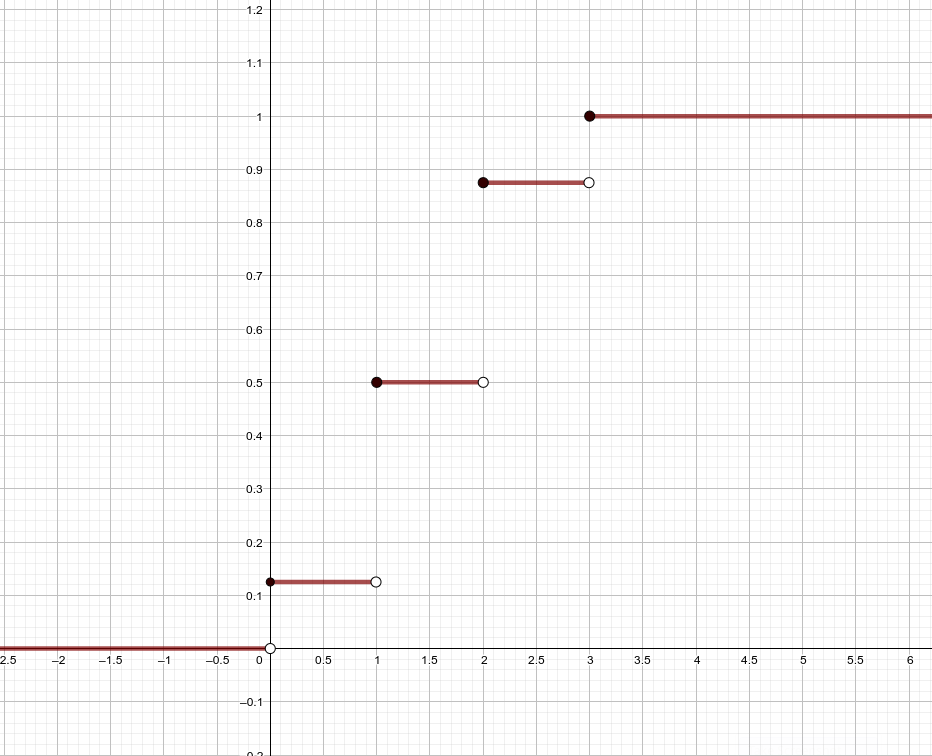
\includegraphics[scale = .3]{Images/CDF.png}
\caption{Notice there is a jump when the random variable takes its value, and the difference where there is a jump is the probability. Also note that the CDF function is defined for the whole $\mathbb{R}$}
\end{figure}

\framebreak

The last figure can be written as a piecewise function

% \begin{columns}
% \begin{column}{0.5\textwidth}
\begin{align*}
F(x)= \begin{cases}0 & : x<0 \\ 
\frac{1}{8} & : 0 \leq x<1 \\ 
\frac{4}{8} & : 1 \leq x<2 \\ 
\frac{7}{8} & : 2 \leq x<3 \\ 
1 & : x \geq 3
\end{cases}
\end{align*}

\medskip

\framebreak

There are $3$ important properties for the CDF, 

\medskip
\begin{itemize}
\item 1) \textbf{Always Non-Decreasing:} If $x_1 \leq x_2$, then $F\left(x_1\right) \leq F\left(x_2\right)$. 

\item[] This makes sense since as we go to the right on the real line, the cumulative probabilities will increase or stay the same, it cannot decrease. 



\medskip
\item 2) \textbf{Right Continuous:} $F(a)=\lim\limits_{x \rightarrow a^{+}} F(x)$.
\item[] This means the right hand limit of the CDF at $a$ is equal to the value of the CDF at $a$ (Do you understand what is a limit?)


\medskip
\item 3) \textbf{At infinity the limits are $0$ and $1$} $\lim\limits_{x \rightarrow-\infty} F(x)=0$ and  $\lim\limits_{x \rightarrow \infty} F(x)=1$.
\item[] This means as we go to the left of the real line, the CDF will approach $0$, and as we go to the right of the real line, the CDF will approach $1$. This makes sense since at $-\infty$ we have no probabilities, and at $+\infty$ we have all probabilities.



\end{itemize}


% \framebreak


% \item  You already know that the idea of understand \alert{quantiles} or \alert{percentiles} are related to cumulative probabilities, from last figure we can calculate,


% \begin{align*}
% P ( X \leq 1.5) = F(1.5) = 4/8
% \end{align*}

% \item In this case we say the number $1.5$ is $4/8 = 0.5^{th}$ \alert{quantile} of the distribution. This means $50\%$ values are below $1.5$. We can also say

% \item We also say $0.253$ is the $60^{th}$ \alert{percentile} of the distribution.

% \item So quantiles and percentiles are same things, when it come to quantiles we write in decimals, for example $0.6$, $0.7$, etc. However for percentile we write $60\%$, $70\%$.

% \item So if someone asks you what is $65\%$ percentile or $.65^{th}$ quantile of the distribution, you should say this is a value below which there are $65\%$ values of the random variable.

% \end{column}
% \begin{column}{0.5\textwidth}  %%<--- here
% \begin{figure}
% 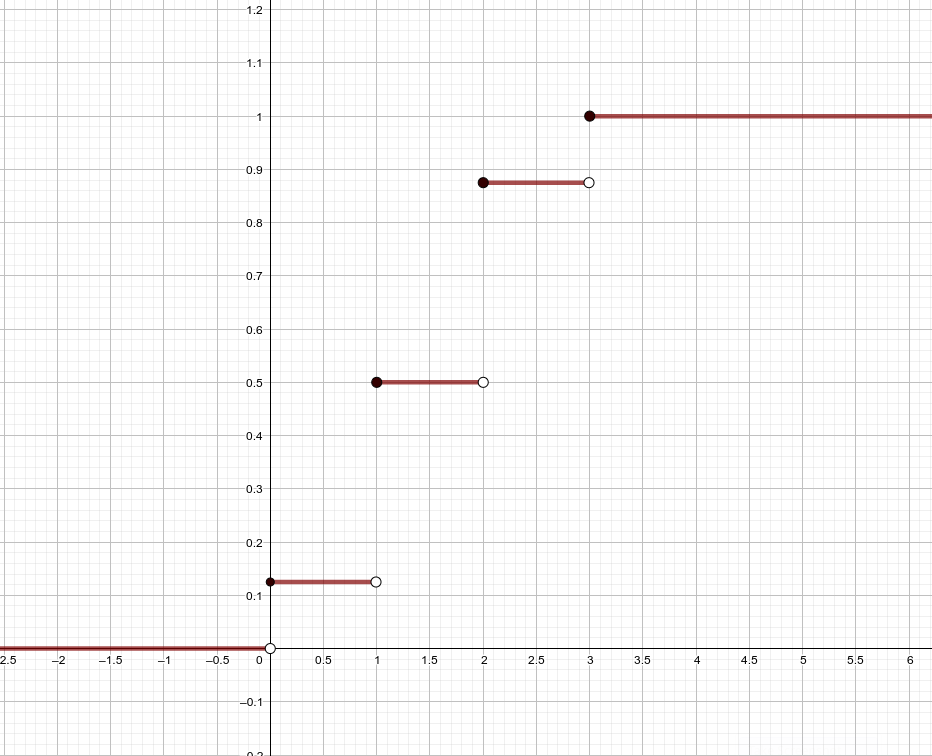
\includegraphics[scale = .2]{Images/CDF.png}
% \caption{Notice there is a jump when the random variable takes its value, and the difference where there is a jump is the probability. Also note that the CDF function is defined for the whole $\mathbb{R}$}
% \end{figure}
% \end{column}
% \end{columns}




% \item \cite{anderson_statistics_2020} motivated the idea of PMF using \alert{empirical discrete distribution}.

% \item The idea is if we know the Population, then we will look for how the values of the random variables are distributed in the population.

% \item Following example will illustrate this idea, this is taken from \cite{anderson_statistics_2020}.


% \item This example gives us a nice intuitive idea, but note that usually we will never know or have access to the population.





\end{itemize}

\end{frame}





\subsection{3. Summary Measures of a Distribution - Expectation $\mathbb{E}(\cdot)$ and Variance $\mathbb{V}(\cdot)$}

\frame{\subsectionpage}

\begin{frame}[allowframebreaks]{Summary Measures}{Expectation $\mathbb{E}(\cdot)$}

\begin{itemize}

\item Now we will learn two important summary measures of the distribution, namely \emph{expected value} and \emph{variance}.

\item Essentially a summary measure is a single number that summarizes the probability distribution of the random variable. 

\item Let's start with \emph{Expected value} or \emph{Expectation} of a random variable. 

\item \alert{An Expected value is a number that gives us an idea about the \alert{central value} of the distribution}, or where most of the values of the random variables are concentrated. 


\item Calculating an Expected Value is very easy, here is the definition,


\begin{varblock}{\Thm{Definition } (Expected Value)}

If $X$ is a \alert{discrete random variable} with values $x_1, x_2, \ldots, x_k$, and it has PMF $f(x)$ then the \alert{Expectation}  or the \alert{Expected Value} of $X$ is defined as 

\begin{align*}
\mathbb{E}(X) = \sum_{i = 1}^{k}x_i \cdot f(x_i)
\end{align*}

We will usually use the notation $\mathbb{E}(\cdot)$ to write the \alert{Expectation} on $X$, and often the number or the expected value is represented with $\mu$

\end{varblock}

\framebreak


\item The formula says for a discrete random variable, if we know the PMF, then calculating Expected value is just \emph{multiplying $x$ with $f(x)$ and then adding them altogether}. 

\item Again if we use the following PMF of a random variable $X$,


\begin{align}
f(x)= \begin{cases} 1/8 & \text { if } x=0 \\ 
3/8 & \text { if } x=1 \\ 
3/8 & \text { if } x=2 \\ 
1/8 & \text { if } x=3 \\ 
0 & \text { otherwise }\end{cases}
\end{align}

\item then we can calculate the expected value as,

\begin{align*}
\mathbb{E}(X) &= \left(0 \times f(0)\right) + \left(1 \times f(1)\right) + \left(2 \times f(2)\right) + \left(3 \times f(3)\right) \\
&=\left(0 \times 1/8\right) + \left(1 \times 3/8\right) + \left(2 \times 3/8\right) + \left(3 \times 1/8\right) = 1.5
\end{align*}

\item So calculation is very easy, now we may ask \emph{what does expected value mean}?


\framebreak

\item Actually Expectation (or Expected value) is a \emph{population average}, or \emph{population mean}, so if we have a population of size $N$, then we can calculate the expected value as,

\begin{align*}
	\frac{\text{sum of all values in the population}}{N}
\end{align*}

\item In expected value we are calculating the same number but the idea is we are \alert{weighting values with their probabilities}... let's explain this with a concrete example


\framebreak

\item \textbf{Example 1: Idea of Expectation }

Suppose we have following \emph{population data} (Careful: It;s not a sample, it's a population) 

\begin{align*}
	\text{Population Data} = \{1, 1, 1, 2, 1, 1, 2, 2, 3, 1, 3, 3, 3, 1\}
\end{align*}

Then in this case population size is $N = 14$, and we can calculate the population average or population mean as

\begin{align*}
	\frac{1 + 1 + 1 + 2 + 1 + 1 + 2 + 2 + 3 + 1 + 3 + 3 + 3 + 1}{14} = \frac{24}{14}  
\end{align*}

Now if we think about a random variable $X$ that can take values $1, 2$ and $3$ then we can think about following \emph{true PMF},

\begin{table}[H]
\centering
	\begin{tabular}{c|c}
$x$ & $f(x)$ \\
\hline $1$ & $7 / 14$ \\
$2$ &  $3/14$  \\
$3$ & $4/14$
\end{tabular}
\end{table}

Now with this PMF we can calculate the expected value as

\begin{align*}
\mathbb{E}(X) &= \left(1 \times f(1)\right) + \left(2 \times f(2)\right) + \left(3 \times f(3)\right) =\left(1 \times 7/14\right) + \left(2 \times 3/14\right) + \left(3 \times 4/14\right) \\
&= \frac{7 + 6 + 12}{14} = \frac{25}{14}
\end{align*}

which gives us the same result as before. 


\framebreak




\item You may ask why we are learning this formula? Why not directly take average of all values? Two reasons,

\medskip
\begin{itemize}

	\item  Almost always we don't have access to the population data, so we cannot calculate the average of all values, but the nice thing about the formula for the expected value is \emph{we can apply the formula when we only know true PMF}. So the formula for expected value gives us the population average even if we don't have all population data and somehow only know true PMF.
	

\medskip
	\item We can extend this idea easily to the continuous case, the idea is replace the $\sum$ with $\int$ (We will see this later)
\end{itemize}

\framebreak


\item \alert{Homework Question:} Suppose from the population data that we have just seen in the last example we take a \emph{random sample} of $5$ numbers (we did \alert{sampling with replacement)}, below is the Population data and the Sample data,

\begin{align*}
	\text{Population Data} &= \{1, 1, 1, 2, 1, 1, 2, 2, 3, 1, 3, 3, 3, 1\} \\
		\text{Sample Data} &= \{1, 1, 2, 2, 3\}
\end{align*}

\item Note here the population size $N = 14$ and the sample size is $n = 5$, now answer following question.

\item Calculate \emph{True PMF and Empirical PMF} (We already solved one)


\item Calculate the Expected Value using the \emph{True PMF} and Direct average? (We already did this)

\item Calculate the sample average using the formula for the sample average.

\item What is the relationship between True PMF and Empirical PMF? 

\item What is the relationship between Expected Value (or Population Average) and Sample Average? 


\end{itemize}



\end{frame}


\begin{frame}[allowframebreaks]{Summary Measure}{Variance $\mathbb{Var}\mathrm{ar}(\cdot)$}

\begin{itemize}
\item Like Expectation, variance is also a summary measure, where the expectation gives an idea of the central value or average, variance gives the idea how \alert{dispersed the values are} (you already know sample variance, but we will learn the population variance formula now)


\begin{varblock}{\Thm{Definition } (Variance)}


If $X$ is a \alert{discrete random variable} with values $x_1, x_2, \ldots, x_k$, and it has PMF $f(x)$ then the \alert{Variance} of $X$ is defined as 

\begin{align*}
\Var(X) = \mathbb{E}\left( \left(X - \mathbb{E}\left(X\right)\right)^2 \right) = \mathbb{E}\left( \left(X - \mu \right)^2 \right) = \sum_{i = 1}^{k}(x_i-\mu)^2 f(x_i)
\end{align*}

where we used $\mu = \mathbb{E}(X)$. Also for the calculated variance we often use the symbol $\sigma^2$.

\end{varblock}

\framebreak

\item First note that, Variance is also an Expectation, but it is an \alert{Expectation of $\left(X - \mu \right)^2$}, NOT $X$. 

\item So what is $\left(X - \mu \right)^2$? Or what is $\left(X - \mu \right)$? Ans: $X - \mu$ is the \emph{deviation of the random variable from its Mean} and $\left(X - \mu \right)^2$ is the \emph{squared deviation}. 

\item So Population Variance is the \alert{Expectation of the squared deviation} (or the population average of the squared deviation!)


\item Let's calculate $\Var(X)$ for the random variable $X$ from the example that we have been using,

\framebreak

\begin{align*}
\Var(X) &= \left( \left(0 - 1.5\right)^2 \times f(0)\right) + \left( \left(1 - 1.5\right)^2 \times f(1)\right) + \\
& \qquad \left( \left(2 - 1.5\right)^2 \times f(2)\right) + \left( \left(3 - 1.5\right)^2 \times f(3)\right) \\
& = \left( \left(-1.5\right)^2 \times 1/8\right) + \left( \left(-0.5\right)^2 \times 3/8\right) + \left( \left(0.5\right)^2 \times 3/8\right) + \left( \left(1.5\right)^2 \times 1/8\right)\\
&=\left(2.25 \times 1/8\right) + \left(0.25 \times 3/8\right) + \left(0.25 \times 3/8\right) + \left(2.25 \times 1/8\right) \\
&= 0.75
\end{align*}

\item Like population average, population variance can be also calculated, using

\begin{align*}
	\frac{\text{sum of all squared deviations in the population}}{N}
\end{align*}

\item But the formula is using the PMF, so same idea like population mean - here we are weighting the squared deviations using the PMF. 


\framebreak

\item So calculating Variance is really easy, if we know PMF we can easily calculate the variance. 

\item The interpretation of the variance is how dispersed the values are.

% \item \textbf{\color{red}A Notational remark:} Often the constant that we get after calculating the variance is denoted by $\sigma^2$. So from now on, if you see $\sigma^2$, you should understand this is a variance like $.75$.

\item As you already know the square root of the variance is called \alert{Standard Deviation}, so if $\sigma^2$ is the Variance, then $\sigma$ is the standard deviation.


\framebreak


\item \alert{Homework Question:} Continuing from the last Homework Question...

\item Calculate the Variance using the \emph{True PMF} and Direct average of the squared deviations? Are they same?

\item Calculate the sample variance using the formula for the sample variance.

\item What is the relationship between Population Variance and Sample Variance?



\end{itemize}

\end{frame}



\subsection{4. Rules of Expectation and Variance}
\frame{\subsectionpage}


\begin{frame}[allowframebreaks]{Rules of Expectation and Variance}

\begin{itemize}


\item We already saw the idea of Expectation, you should always keep the following picture in your mind, that expectation works on random variables, not on number, and the result of Expectation is a constant.


\begin{figure}
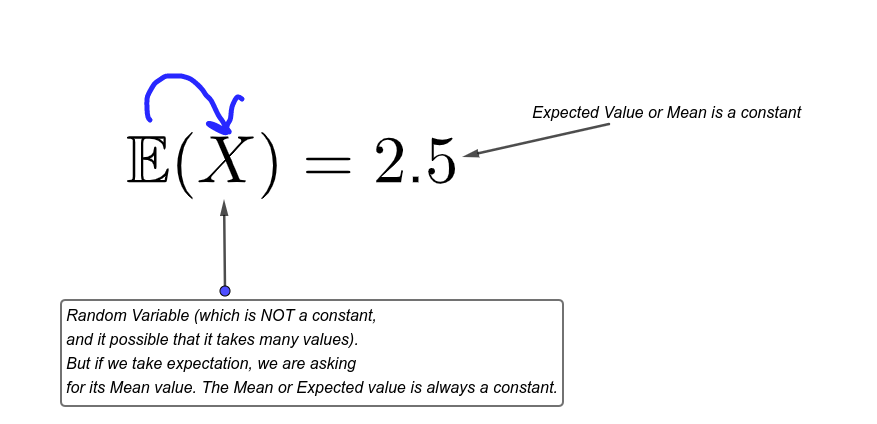
\includegraphics[scale = .5]{Images/RV_1.png}
\end{figure}


\framebreak

\item Now we consider a slightly different problem, we ask what is 

{\huge{
\vspace*{-.5cm}
\begin{align*}
\mathbb{E}(X^2) \text{ or } \mathbb{E}(X^3)  \text{ or } \mathbb{E}(3 + 2X) \text{ ??? }
\end{align*}
}}

\item Note that $X^2$, $X^3$ or $3 + 2X$ are all functions of random variable $X$. 

\item So now our question is \emph{for functions $X^2$, $X^3$ or $3 + 2x$, what are the expected values}. First of all note that \emph{any function of a random variable is also a random variable}. 

\item It turns out that for a function $g(X)$ in this case we can calculate $\mathbb{E}(g(X))$ by using the distribution of $X$, the idea is the following,

\begin{align*}
\mathbb{E}(g(X)) &= \sum_{i = 1}^{k} g(x_i) f(x_i) 
\end{align*}

\item This rule has an interesting name, it is called - \alert{Law of the unconscious Statistician} or in short \alert{LOTUS} 

\item Why this name? Since we just used the distribution of $X$ blindly...

\framebreak

\item Applying this rule we can easily calculate expectation of All functions of $X$.

\begin{align*}
	\mathbb{E}(X^2) &= \sum_{i = 1}^{k} x_i^2 f(x_i) \\
	\mathbb{E}(X^3) &= \sum_{i = 1}^{k} x_i^3 f(x_i) \\
	\mathbb{E}(3 + 2X) &= \sum_{i = 1}^{k} (3 + 2x_i) f(x_i) \\
\end{align*}

\item In the last case, we have a simpler way to calculate, we can use the following rule,

\begin{align*}
		\mathbb{E}(3 + 2X) &= 3 +  2 \mathbb{E}(X) 
\end{align*}


\item This is called the \emph{linearity of expectation}, and it is a very important rule. In general the rule says,

\begin{align*}
	\mathbb{E}(a + bX) &= a + b \mathbb{E}(X)
\end{align*}

\item where $a$ and $b$ are any constants. 

\item We will see the proof of this rule, but before let's learn some rules for the summation...

\framebreak


	\begin{block}{\Thm{Rules }~ Algebra Rules for Summation}

	\begin{itemize}
		\item \alert{Sum and Difference Rule}:

			$$
			\sum\limits_{i=1}^n\left(x_i \pm y_i\right)=\sum\limits_{i=1}^n x_i \pm \sum\limits_{i=1}^n y_i
			$$


		\item \alert{Constant Multiple Rule:} For any constant or fixed number $c$

			$$
			\sum\limits_{i=1}^n c \;x_i=c \cdot \sum\limits_{i=1}^n x_i
			$$


		\item \alert{Constant Value Rule:} For any constant or fixed number $c$
		
		$$
		\sum\limits_{i=1}^n c=n \cdot c
		$$

	\end{itemize}

			
	\end{block}

	\item These rules are very useful when it comes to doing summation. Let's see some examples, you will see  more examples in the homework.


	\framebreak

	\item \Thm{Example~}~

	\begin{itemize}
	\item[(a)] $\sum\limits_{k=1}^n\left(3 k-k^2\right)=3 \sum\limits_{k=1}^n k-\sum\limits_{k=1}^n k^2$
	\item[(b)] $\sum\limits_{k=1}^n\left(-a_k\right)=\sum\limits_{k=1}^n(-1) \cdot a_k=-1 \cdot \sum\limits_{k=1}^n a_k=-\sum\limits_{k=1}^n a_k$
	\item[(c)]

		\begin{align*}
			\sum\limits_{k=1}^3(k+4) & =\sum\limits_{k=1}^3 k+\sum\limits_{k=1}^3 4 \\
		& =(1+2+3)+(3 \cdot 4) \\
		& =6+12=18
		\end{align*}



	\item[(d)] $\sum\limits_{k=1}^n \frac{1}{n}=n \cdot \frac{1}{n}=1$


	\item [(e)] (Do this!)

	\begin{align*}
	\frac{1}{n}\sum_{i = 1}^{n} (x_i - \bar{x})^2  = \frac{1}{n}\sum_{i = 1}^{n} x_i^2 - \bar{x}^2
	\end{align*} 

	notice $\frac{1}{n}\sum_{i = 1}^{n} (x_i - \bar{x})^2$ is also a formula for sample variance, in fact when $n$ is very large, there is not so much difference between $\frac{1}{n}\sum_{i = 1}^{n} (x_i - \bar{x})^2$ and $\frac{1}{n-1}\sum_{i = 1}^{n} (x_i - \bar{x})^2$



	\end{itemize}



\end{itemize} 



Now let's apply the rules to see whether the linearity of expectation is correct...




\begin{align}
\mathbb{E}[a+b X] &= \sum_{i = 1}^{k} (a + bx_i) f(x_i)\\
&=\sum_{i=1}^{k} a  f(x_i) + \sum_{i=1}^{k} b \;x_i \; f(x_i) \\
&=a \sum_{j=1}^{k} f(x_i)+b \sum_{j=1}^{n} x_i f(x_i) \\
&=a+b \mathbb{E}[X]
\end{align}



Notice the \emph{linearity of expectation} rule simply says, 1) Expectation of a constant is always constant and 2) If constant is multiplied with a random variable, we can always pull it out from the Expectation.


\medskip

Linearity is actually remarkable property of Expectation, later we will see that we can apply this property for many random variables together.

\framebreak

Notice interestingly if you look at the formula for the Variance, it already has the idea of LOTUS, since 

\begin{align*}
	\Var(X) &= \mathbb{E}\left[ \left(X - \mu \right)^2 \right] \\
	& = \sum_{i = 1}^{k} \left(x_i - \mu\right)^2 f(x_i) \\
\end{align*}

\medskip

But interestingly using \emph{linearity of expectation} we can get another formula for variance,

\begin{align*}
	\Var(X) &= \mathbb{E}\left[ \left(X - \mu \right)^2 \right] \\
	&= \mathbb{E}\left[X^2 - 2X\mu + \mu^2\right] \\
	&= \mathbb{E}\left[X^2\right] - 2\mu \mathbb{E}\left[X\right] + \mu^2 \\
	&= \mathbb{E}\left[X^2\right] - 2\mu^2 + \mu^2 \\
	&= \mathbb{E}\left[X^2\right] - \mu^2 = \mathbb{E}\left[X^2\right] - \left(\mathbb{E}\left[X\right]\right)^2
\end{align*}

\medskip

So both are valid formulas, and you can use any of them. 


\framebreak

So this means for the population variance, we have two equivalent ways of writing variance, and they are, 

\begin{align*}
	\Var(X) = \mathbb{E}\left[ \left(X - \mu \right)^2 \right] = \mathbb{E}\left[X^2\right] - \left(\mathbb{E}\left[X\right]\right)^2
\end{align*}

\medskip
and for the sample variance with $\frac{1}{n}$, we have

\begin{align*}
	S^2 = \frac{1}{n}\sum_{i = 1}^{n} (x_i - \bar{x})^2  = \frac{1}{n}\sum_{i = 1}^{n} x_i^2 - \bar{x}^2
\end{align*}

\framebreak

\begin{itemize}

\item Now we can also ask what is $\Var(a + bX)$?

\item It turns out that in this case, we can use the following rule,



\begin{align*}
\Var(a + bX) = \Var(a) + \Var(bX) = 0 + b^2 \Var(X) = b^2 \Var(X)
\end{align*}


\item where $\Var(a) = 0$, since $a$ is not a 	random variable, and it has a fixed value, so no variance.


\item What about $\Var(bX)$? This is also easy, we can check this using the definition of variance and the linearity of expectation,

\begin{align*}
\Var(bX) &= \mathbb{E}\left[ \left(bX - \mathbb{E}\left[bX\right]\right)^2 \right] \\
&= \mathbb{E}\left[ \left(bX - b\mathbb{E}\left[X\right]\right)^2 \right] \\
&= \mathbb{E}\left[ \left(b \left(X - \mathbb{E}\left[X\right]\right)\right)^2 \right] \\
&= \mathbb{E}\left[ b^2\left(X - \mathbb{E}\left[X\right]\right)^2 \right] \\
&= b^2 \mathbb{E}\left[ \left(X - \mathbb{E}\left[X\right]\right)^2 \right] \\
&= b^2 \Var(X)
\end{align*}

\framebreak

\item This gives us two following rules for the linear function of $X$, that is 

\begin{align*}
\mathbb{E}(a + bX) &= a + b \mathbb{E}(X) \\
\Var(a + bX) &= b^2 \Var(X) \\
\end{align*}





\framebreak




\item[] \alert{Homework Question:}
\medskip

\item Suppose we have a random variable $X$ that takes 3 values, 1, 2, and 3 with following PMF, 

\begin{table}[H]
\centering
	\begin{tabular}{c|c}
$x$ & $f(x)$ \\
\hline $1$ & $1 / 4$ \\
$2$ &  $1/2$  \\
$3$ & $1/4$
\end{tabular}
\end{table}


\item Calculate Expected Value and Variance using the PMF. 

\item Now using Linearity of Expectation and LOTUS, calculate $\mathbb{E}(2 + X^2)$, $\mathbb{E}(3X + X^3)$ and $\mathbb{E}(3 + 2X)$.

\item Calculate $\Var(3 + 2X)$ using the rules of variance.


\end{itemize}







\end{frame}


\section{Parametric Distributions : Discrete}
\frame{\sectionpage}

\subsection{1. Discrete Uniform}
\frame{\subsectionpage}

\begin{frame}[allowframebreaks]{Parametric Distribution}{Discrete Uniform Distribution}

\begin{itemize}


\item There are many theoretical discrete distributions, these are often called parametric distributions.

\item The idea of parameter is - it's simply a number (or a set of numbers) such that if we change the number, the distribution will change. 

\item There are many parametric discrete distributions, and we will see some of them in this course. 

\begin{itemize}
	\item \emph{Discrete Uniform Distribution}, 
	\item \emph{Bernoulli distribution}, 
	\item \emph{Binomial distribution} and 
	\item \emph{Poisson distribution}.
\end{itemize}

\item Let's start with \alert{Discrete Uniform Distribution}, and will talk about other distributions in coming sections.

\framebreak


\item \alert{Discrete Uniform Distribution} is similar to the idea of equally likely outcomes but this is for the values of the random variable.


\begin{varblock}{\Thm{Definition } (Discrete Uniform Distribution)}
If $X$ can take values $ x_1, x_2, \ldots, x_k$ then we say $X$ follows \alert{Discrete Uniform} distribution with parameter $\{x_1, x_2, \ldots, x_k\}$ if the PMF of $X$ can be written as,

\begin{align*}
f(x) = \left\{\begin{array}{ll}
\frac{1}{k} & \text { for } x=x_1,x_2, \ldots, x_k \\
0 & \text { otherwise }
\end{array}\right\}
\end{align*}
We write this as $X \sim \mathrm{DUnif}\{x_1, x_2, \ldots, x_k\}$.
\end{varblock}

\item Here parameter determines which specific Uniform Distribution we have and changing the parameter will change the distribution. It will be still a discrete uniform distribution but the distribution will change (see example in the next slide).


\item Note that $X$ can take values in any finite set, the idea of a discrete uniform random variable is the \emph{values will all have equal probabilities}. Let's see a real life example.


\framebreak

\item  Suppose everyday your brother can give you $10$, $20$ or $30$ taka and he might give you any of the three amounts with equal probability. 


\item So Let $X$ be a random variable that represents the amount of money, then $X$ follows a discrete uniform distribution with parameter $\{10, 20, 30\}$, we write $X \sim \mathrm{DUnif}\{10, 20, 30\}$ and the PMF of $X$ is

\begin{table}[H]
\centering
	\begin{tabular}{c|c}
$x$ & $f(x)$ \\
\hline $10$ & $1 / 3$ \\
$20$ &  $1/3$  \\
$30$ & $1/3$
\end{tabular}
\end{table}

\item How does it look like?

\begin{figure}
	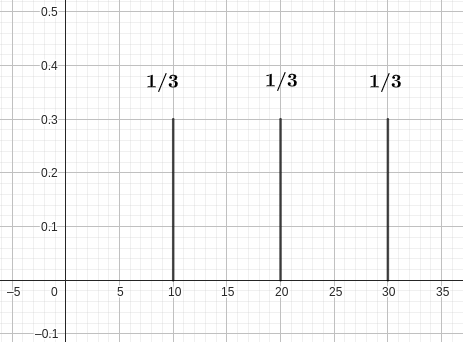
\includegraphics[scale = .4]{Images/DiscreteUniform.png}
\end{figure}

\item Notice here parameter is $\{10, 20, 30\}$, so if we change the parameter, for example, if we change the parameter to $\{10, 20, 30, 40\}$, then the distribution will change.


\item For the following Discrete Uniform PMF, We can easily calculate the Expected Value and Variance.

\begin{table}[H]
\centering
	\begin{tabular}{c|c}
$x$ & $f(x)$ \\
\hline $10$ & $1 / 3$ \\
$20$ &  $1/3$  \\
$30$ & $1/3$
\end{tabular}
\end{table}

\item Using the formula for the expected value we can calculate,

\begin{align*}
\mathbb{E}(X) &= \left(10 \times f(10)\right) + \left(20 \times f(20)\right) + \left(30 \times f(30)\right) \\
&= \left(10 \times 1/3\right) + \left(20 \times 1/3\right) + \left(30 \times 1/3\right) \\
&= \left(10 + 20 + 30\right) \times \frac{1}{3} = \frac{60}{3} = 20
\end{align*}


\item Using the formula for the variance we can calculate,

\begin{align*}
\Var(X) &= \mathbb{E}\left( \left(X - \mathbb{E}\left(X\right)\right)^2 \right) = \mathbb{E}\left( \left(X - 20\right)^2 \right) \\
&= \left( \left(10 - 20\right)^2 \times f(10)\right) + \left( \left(20 - 20\right)^2 \times f(20)\right) + \\
& \qquad \left( \left(30 - 20\right)^2 \times f(30)\right) \\
&= \left( \left(-10\right)^2 \times 1/3\right) + \left( \left(0\right)^2 \times 1/3\right) + \left( \left(10\right)^2 \times 1/3\right) \\
&= \left(100 \times 1/3\right) + \left(0 \times 1/3\right) + \left(100 \times 1/3\right) \\
&= \left(100 + 0 + 100\right) \times \frac{1}{3} = \frac{200}{3} = 66.67
\end{align*}




\end{itemize}

\end{frame}



\subsection{2. Bernoulli and Binomial Distribution}
\frame{\subsectionpage}



\begin{frame}[allowframebreaks]{Bernoulli \& Binomial Random Variables}


\begin{itemize}

\item If a random variable $X$ only has two values $0$ and $1$, we call the random variable a \alert{Bernoulli Random variable}, and its distribution is known as \alert{Bernoulli distribution},  some examples could be,

\begin{itemize}
\item When we toss a coin, a random variable $X = 1$ means head, $X = 0$ means tail.

\item When we sample then Gender of a person, So $X = 1$ means female, and $X = 0$ means male 

\item When we call a customer, a Random Variable $X$ could be such that $X = 1$ means picked up the call, $X = 0$ means didn't pickup.

\item And so on.... 


\end{itemize}




\item In practice or in real life scenario, when you have possible data with $0, 1, 0, 1, 0, 1$, you can think about these are values of some Bernoulli random variables. So in any experiment, when we have only two possible outcomes we can think about modeling that experiment using a Bernoulli random variable. For a Bernoulli random variable, if $X = 1$, we often call it \emph{``success''} and if $X = 0$, we often call it ``failure''. Here is the formal definition.

\framebreak


\begin{varblock}{\Thm{Definition } (Bernoulli Distribution)}
 A random variable $X$ is said to follow Bernoulli distribution with parameter $p$ if the PMF of $X$ can be written as,

\begin{align*}
f(x) &= p^x {(1 - p)}^{1-x}, \quad \text{ when } x = 0, 1 \\
&  = 0, \quad \text{otherwise}
\end{align*}

where $0<p<1$. We write $X \sim \operatorname{Bern}(p)$ to represent $X$ follows Bernoulli Distribution with parameter $p$

\end{varblock}



\item Note that, because of this PMF, we have $\mathbb{P}(X=1)=f(1) = p$ and $\mathbb{P}(X=0)= f(0) = 1-p$.

\item Notice, the parameter $p$ controls the probability and hence controls the distribution of the random variable. For example, if $X \sim \operatorname{Bern}(0.3)$, this automatically means $\mathbb{P}(X = 1) = 0.3$ and $\mathbb{P}(X = 0) = 0.7$. Here is how the PMF will look like for different parameters $p$,

\begin{figure}
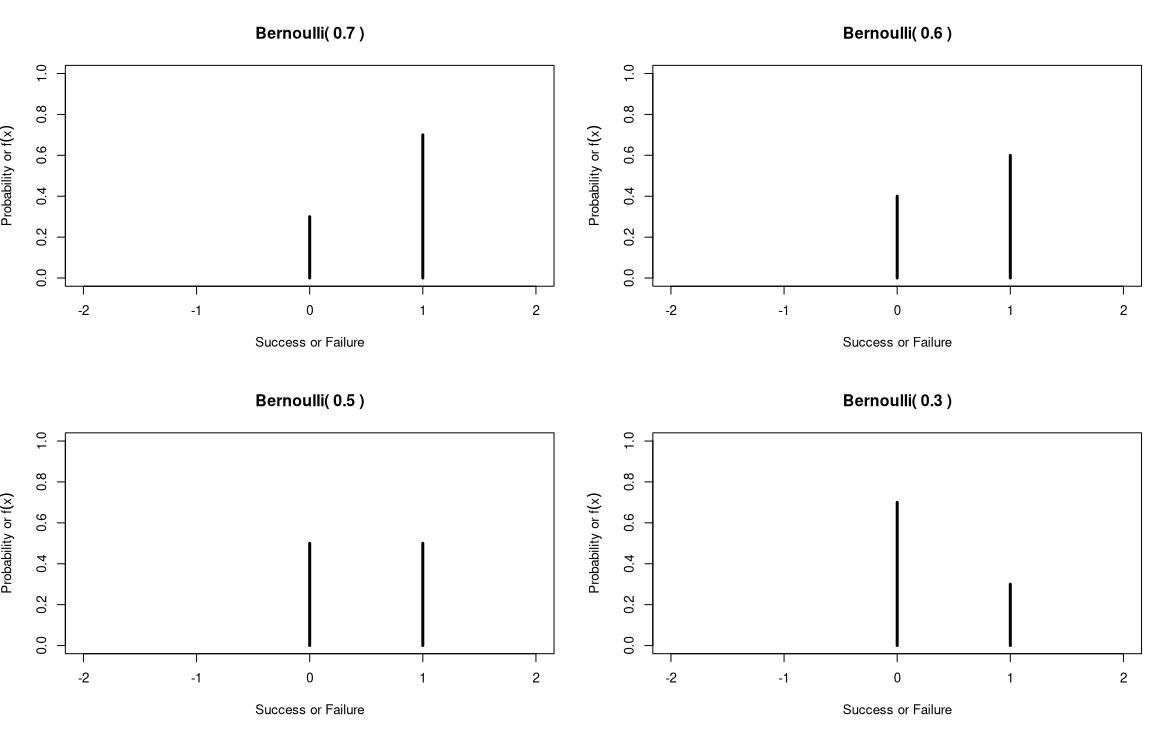
\includegraphics[scale = .3]{Images/BernoulliDistPMF.png}
\end{figure}


\item Because we have the PMF we can also calculate the Expected Value and Variance of a Bernoulli random variable.

\item If you do the calculation, then you should get $\mathbb{E}(X) = p$ and $\Var(X) = p (1-p)$ (please do the calculation!)

\framebreak

\item Now let's talk about Binomial distribution, The Binomial distribution comes when we perform \emph{more than one independent Bernoulli experiments}.


\item Here is the story - Suppose now we perform $n$ independent Bernoulli experiments (or \emph{Bernoulli trials}, like tossing a coin) with parameter $p$. 

\item If $X$ is a random variable which represents the total number of success out of the $n$ trials, then we say the random variable $X$ follows Binomial distribution with parameter $n$ and $p$.

\item You already know the example, ... number of heads ... recall..

\item Here is the formal definition

\framebreak

\begin{varblock}{\Thm{Definition } (Binomial Distribution)}
	Suppose that $n$ independent Bernoulli trials are performed, each with the same success probability $p$, we say $X$ follows Binomial distribution with parameters $n$ and $p$ if the PMF of $X$ can be written as 

\begin{align*}
f(x)&=\left(\begin{array}{l}
n \\
x
\end{array}\right) p^x(1-p)^{n-x} \quad \text{ for } x = 0, 1, 2, \ldots, n \\
&= 0, \text{ otherwise}
\end{align*}

We write $X \sim \operatorname{Bin}(n, p)$ to mean that $X$ has the Binomial distribution with parameters $n$ and $p$, where $n$ is a positive integer and $0<p<1$. 

\end{varblock}

\framebreak

\item Notice here $x$ is the value of the random variable where $x$ can be $0, 1, 2, \ldots, n$. The PMF looks very similar to Bernoulli PMF, except we have a combination term, recall 

\begin{align*}
	\left(\begin{array}{l}
n \\
x
\end{array}\right) = \Combine[n]{x} = \frac{n!}{x! (n-x)!}
\end{align*}

\item Question is why is this coming? 


\item Here is a short answer, the experiment consisting of $n$ independent Bernoulli trials produces a sequence of successes and failures. The probability of any specific sequence of $x$ successes and $n-x$ failures is $p^x(1-p)^{n-x}$. There are $\Combine[n]{x}$ such sequences.



\item We can also calculate the Mean and the Variance of the Binomial distribution. \alert{If $X \sim \textrm{Bin}(n, p)$, then $\mathbb{E}(X) = np$ and $\Var(X) = np(1-p)$}, where do we get this? You can see the proof in the next page. However there is an easy trick that is you remember Binomial is the sum $n$ independent Bernoulli trials (Let's do it using easy trick!)


\item The easy trick is applying linearity of expectation... and for variance applying the idea of independence.... from Bernoulli...

\framebreak


\item If $X \sim \mathrm{Bin}(n, p)$, then applying the formula for Expectation

$$
\mathbb{E}(X)=\sum_{x=0}^n x f(x)=\sum_{x=0}^n x\left(\begin{array}{l}
n \\
x
\end{array}\right) p^x q^{n-x} .
$$

\item Note here we wrote $q = (1-p)$. Also note that we have $x\left(\begin{array}{c}n \\ x\end{array}\right)=n\left(\begin{array}{c}n-1 \\ x-1\end{array}\right)$, so
$$
\begin{aligned}
\sum_{x=0}^n x\left(\begin{array}{l}
n \\
x
\end{array}\right) p^x q^{n-x} &=n \sum_{x=0}^n\left(\begin{array}{c}
n-1 \\
x-1
\end{array}\right) p^x q^{n-x} \\
&=n p \sum_{x=1}^n\left(\begin{array}{c}
n-1 \\
x-1
\end{array}\right) p^{x-1} q^{n-x} \\
&=n p \sum_{j=0}^{n-1}\left(\begin{array}{c}
n-1 \\
j
\end{array}\right) p^j q^{n-1-j} \\
&=n p .
\end{aligned}
$$

Then \emph{we get $\mathbb{E}(X) = np$, similarly we can derive the variance is $\mathbb{V}\mathrm{ar}(X) = np(1-p)$ (I am skipping the proof). Again the easy trick is to apply Binomial - Bernoulli relation}.


\item Here is how the PMF will look like for two Binomial distributions, with same $n = 3$ but different $p$.

\begin{figure}
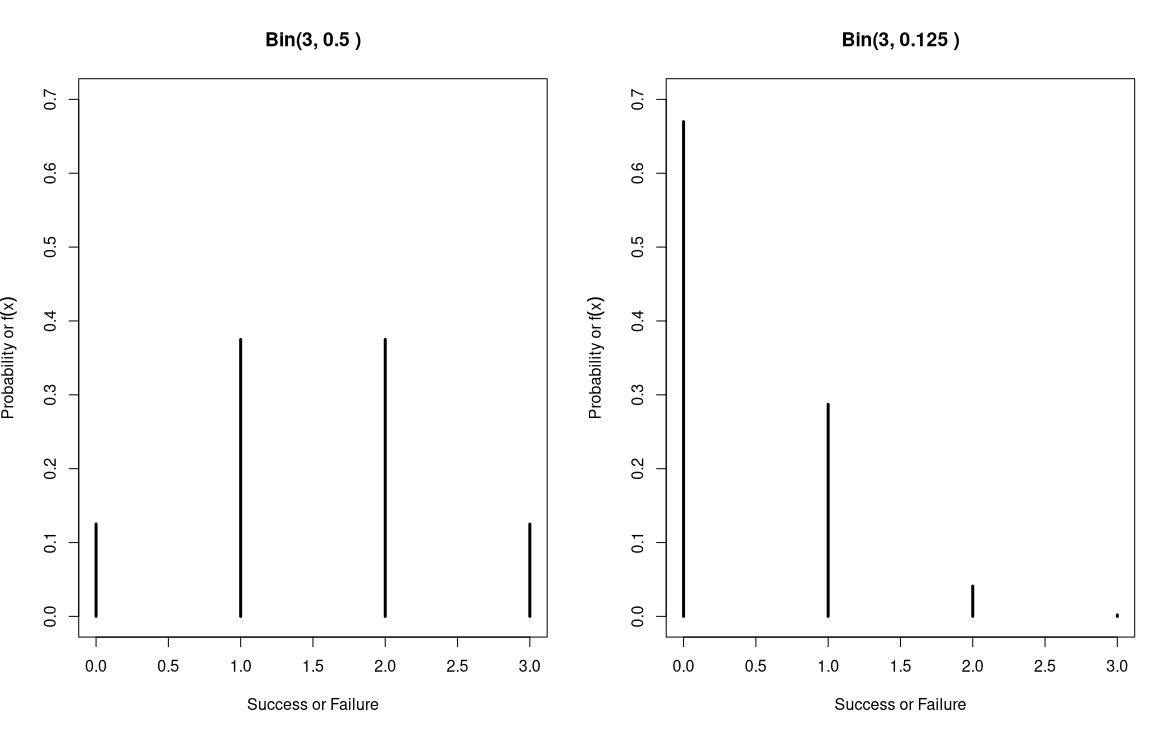
\includegraphics[scale = .3]{Images/Binomial-1.png}
\caption{On the left we have the PMF of $X \sim \textrm{Bin}(3, 0.5)$ and on the right we have $X \sim \textrm{Bin}(3, 0.125)$.  }
\end{figure}



\begin{figure}
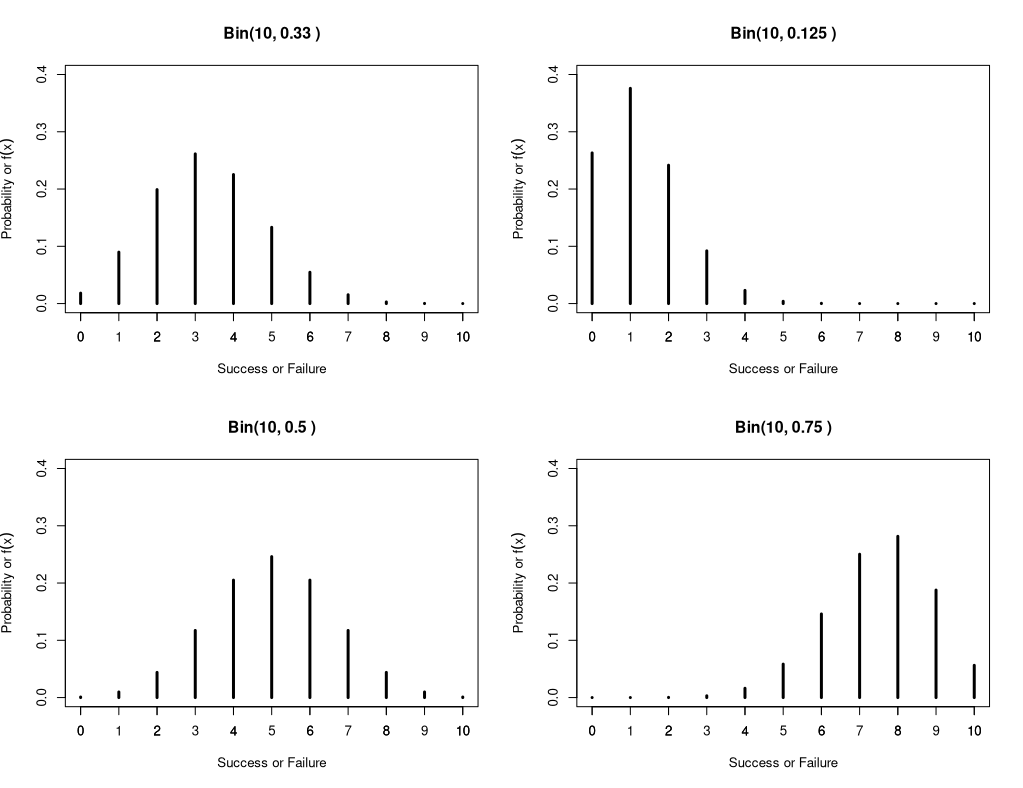
\includegraphics[scale = .3]{Images/Binomial-2.png}
\caption{From top left, we have the PMF of $X \sim \textrm{Bin}(10, 0.33)$, then right $X \sim \textrm{Bin}(10, 0.125)$, then bottom left $X \sim \textrm{Bin}(10, 0.5)$ and right $X \sim \textrm{Bin}(10, 0.75)$  }
\end{figure}


\item Binomial distribution comes in many forms in real life, you should always remember the essential structure - \emph{that is tossing $n$ independent coins and then the random variable is the number of success out of $n$}.

\item Here are some examples where we can think about a Binomial random variable.

\begin{itemize}
\item  Random experiment: Calling $n$ people. Random variable $X$ will represent how many people will answer the call.

\item Random experiment: $n$ students registered for a course. Random variable $X$ will represent how many students will finish it.

\item Random experiment: Randomly asking $5$ people whether they are satisfied with the transportation system of Bangladesh. Random variable is number of people who said "yes"! 

\item And there are more examples in \cite{anderson_statistics_2020}.


\end{itemize}

\item Notice two important assumptions for the Binomial random variable is, 1) all trials are independent and 2) all trials happens with same probability. Only in these cases you can think about the random variable is Binomial.



\end{itemize}


\end{frame}

 


\section{Continuous Random Variables}
\frame{\sectionpage}

\subsection{1. Probability Distribution and the idea of PDF}
\frame{\subsectionpage}




\begin{frame}[allowframebreaks]{Probability Distributions}{Idea of PDF}

\begin{itemize}


\item Now let's talk about continuous distributions. How do we extend the idea of PMF, Expectation and Variance for continuous random variables?


\item Recall histogram, the idea of histogram is very similar to PMF, but the difference is PMF is for discrete random variable and histogram is for continuous random variable where we have a lot of data points.


\item In the histogram, we have some bins and we count the number of data points in each bin and then we divide by the total number of data points to get the relative frequency in each bin.


\item What if we have a lot of data points and make the size of the bins very small? 

\item Can you visualize what happens? We might get a very smooth curve like this. it's called PDF


\begin{figure}
\centering
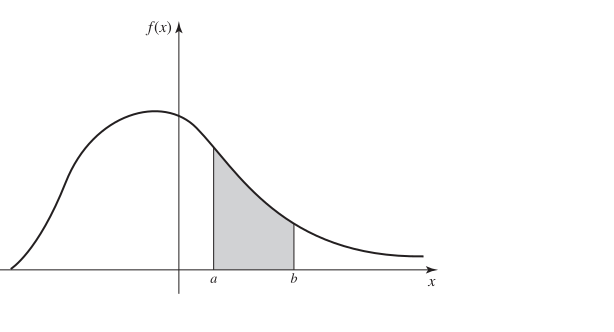
\includegraphics[scale = .3]{Images/PDF_1.png}
\end{figure}

\framebreak

\item Similar to PMF, for continuous random variable we have another function called \emph{probability density function (or PDF)} to calculate the probabilities.



\item Here the idea is if we know the \emph{pdf of the random variable}, then we can calculate the probability of any interval in $\mathbb{R}$ with integral. For example here is a PDF, it's a function of $x$,

\begin{figure}
\centering
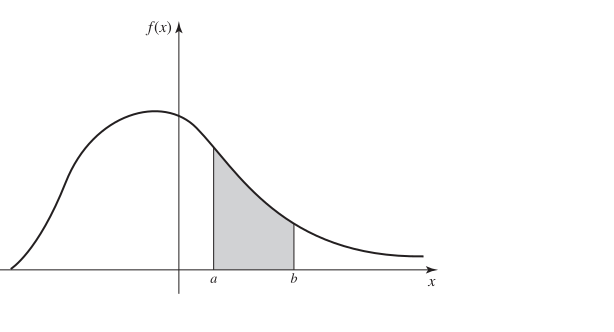
\includegraphics[scale = .3]{Images/PDF_1.png}
\caption{ Here the shaded area is the probability of a random variable $X$ taking value between $a$ and $b$, so this means the shaded area is $\mathbb{P}(a \leq X \leq b]) = \int_{a}^{b} f(x) dx$}
\end{figure}

\item Now how do we calculate probability of $X$ takes value in the interval $[a, b]$, the idea is we can simply integrate, so $\mathbb{P}(a \leq X \leq b) = \int_{a}^{b} f(x) dx$, since integration meas finding area under the curve, so the probability of $X$ takes value in $[a, b]$ = area under the curve in the interval $[a, b]$.

\item So you should remember for a continuous random variable $X$ with density function $f(x)$

\begin{align*}
	\text{Probability of $X$ taking value in the interval } [a, b] &= \mathbb{P}(a < X < b)\\
	&= \int_{a}^{b} f(x) dx \\
	&= \text{area under the density function} 
\end{align*}

\medskip

Here is the definition of a density function ..

\framebreak

\begin{varblock}{\Thm{Definition} (Probability Density Function (PDF))}

If $X$ is a continuous random variable then a \alert{nonnegative} function $f(x)$ on $\mathbb{R}$ is called the probability density function (in short PDF) of $X$ if for any interval, for example $[a, b]$, we have

\begin{align*}
\mathbb{P}(X \in [a, b]) =   \mathbb{P}(a \leq X  \leq b) = \int_{a}^{b} f(x) d x
\end{align*}

and it satisfies $\int_{-\infty}^{\infty} f(x) dx = 1$ (the density function should be integrated to $1$).


\end{varblock}



\medskip




\item  Note we can also calculate, $\mathbb{P}(X \geq a)=\int_a^{\infty} f(x) d x$ and $\mathbb{P}(X \leq b)=\int_{-\infty}^b f(x) d x$. 
\item Notice a PDF must satisfy two conditions, 

\begin{itemize}
	\item 1. $f(x) \geq 0$, it is always non-negative for any value of $x$ 
	\item 2. $\int_{-\infty}^{\infty} f(x) dx = 1$ (if we integrate for all values it will be $1$)
\end{itemize}

\framebreak

\item The idea of a density function for a continuous random variable $X$ is same as the the probability mass function for a  discrete random variable.


\item For continuous random variable we will learn 3 important continuous distributions, 

\begin{itemize}
	\item \emph{Uniform distribution}, 
	\item \emph{Normal distribution} and 
	\item \emph{Exponential distribution} 
\end{itemize}


\item Let's see the uniform distribution now. Notice this is a continuous uniform distribution, the idea is very similar to discrete, but it's for a continuous random variable.

\framebreak

\item Intuitively, a Uniform random variable on the interval $(a, b)$ is a completely random number between $a$ and $b$. Here is the formal definition,

\begin{varblock}{Uniform Distribution}
A continuous random variable $X$ is said to follow the \alert{Uniform Distribution} on the interval $(a, b)$ if its PDF is

$$
f(x)= \begin{cases}\frac{1}{b-a} & \text { if } a<x<b, \\ 0 & \text { otherwise. }\end{cases}
$$

We denote this by $X \sim \operatorname{Unif}(a, b)$, and we have  

\begin{align*}
\mathbb{E}(X) &= \frac{a+b}{2} \\
\Var(X) &= \frac{(b-a)^2}{12}
\end{align*}

	
\end{varblock}


\item Let's see a real life example, (this is adapted from \citet{anderson_statistics_2020})

\framebreak

\item Think about a random variable $X$ that represents the flight time of an airplane traveling from Dhaka to Chittagong. Suppose the flight time can be any value in the interval from 60 minutes to 90 minutes. With every 1-minute interval being equally likely, we can think the random variable $X$ follows a uniform probability distribution, so $X \sim \operatorname{Unif}(60, 90)$.

\item Now because $\frac{1}{90 - 60} =  \frac{1}{30}$, the PDF of $X$ can be written as 

\begin{align*}
	f(x) = \begin{cases}
		 \cfrac{1}{30} & \text{ if } 60 \leq x \leq 90, \\
		\\
		0 & \text{ otherwise}
	\end{cases}
\end{align*}

\item  How does it look like?

\begin{figure}[H]
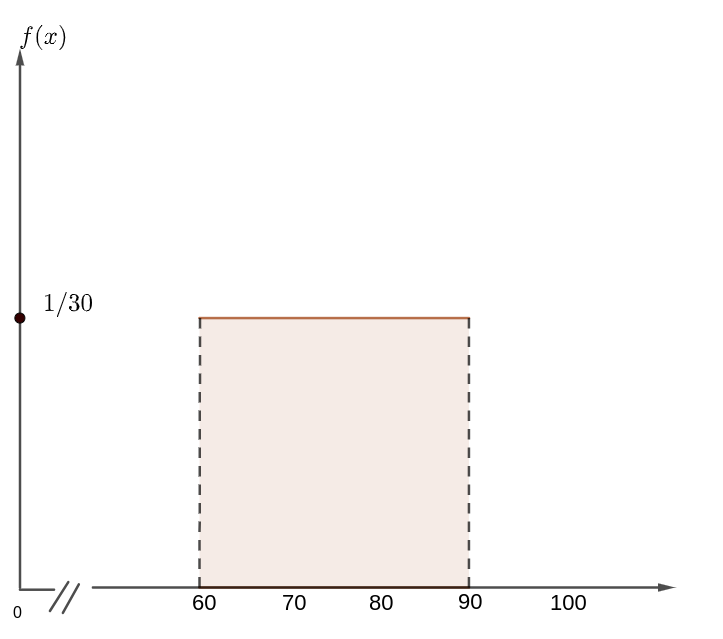
\includegraphics[scale = .2]{Images/Cont_Uniform.png}
	
\end{figure}


\item Now with this density we can calculate the probability of $X$ taking value in any interval, for example, 

\begin{align*}
	\mathbb{P}(65 < X < 75) = \int_{65}^{75} f(x) dx = \int_{65}^{75} \frac{1}{30} dx = \frac{1}{30} [x]_{65}^{75} = \frac{1}{30} (75 - 65) = \frac{10}{30} = \frac{1}{3}
\end{align*}

\item So this means there is $1/3$ probability that the flight time will be between 65 minutes and 75 minutes.

\framebreak

\item Note that this also shows probability is an area under the curve, in the following this is the shaded area,

\begin{figure}
 	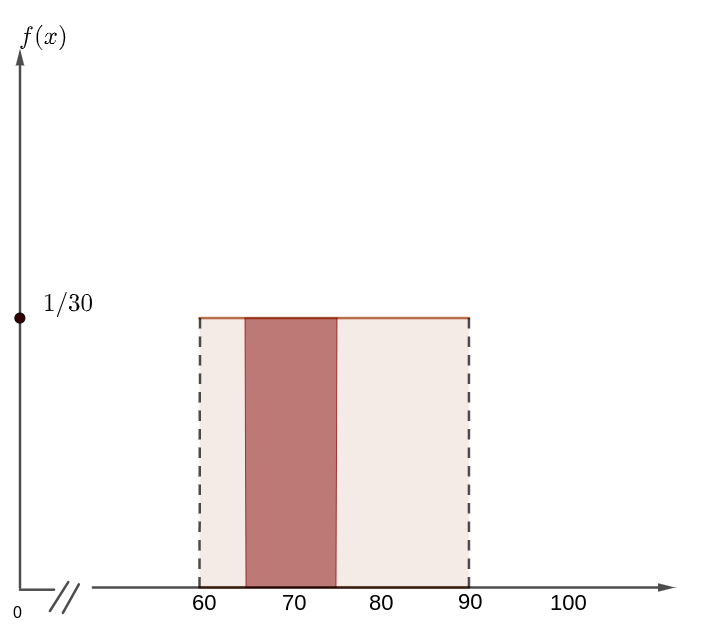
\includegraphics[scale = .2]{Images/Cont_Uniform_area.png}
 \end{figure} 

\item Since in this case the area is a rectangle, we can apply the formula for area of a rectangle to calculate the area, which is $10 \times \frac{1}{30} = \frac{10}{30} = \frac{1}{3}$.


\item Similarly, we can calculate $\mathbb{P}(70 \leq X \leq 80) = \frac{1}{3}$, $\mathbb{P}(75 \leq X \leq  85) = \frac{1}{3}$ and so on.


\item In general for $X \sim \operatorname{Unif}(a, b)$ we can calculate $\mathbb{P}(c \leq X \leq d) = \frac{1}{b-a} \times (d - c)$

\framebreak

\item Here is another example of a PDF (this is not uniform), suppose we have a random variable $X$ takes value in $[0, 1]$, with following PDF,

$$
f(x)= \begin{cases}2 x & \text { for } 0<x<1 \\ 0 & \text { otherwise. }\end{cases}
$$

\begin{figure}
	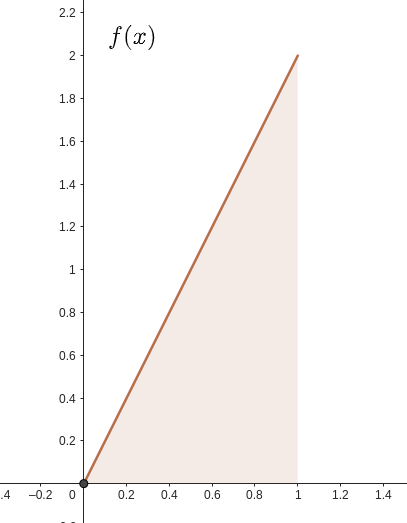
\includegraphics[scale = .25]{Images/cont_pdf.png}
\end{figure}


\item Is this a valid PDF? YES! note it satisfy two conditions

\begin{itemize}
\item $f(x) \geq 0$ for all $x$
\item $\int_{0}^{1} f(x) dx = \int_{0}^{1} 2x dx = 1  $ 
\end{itemize}

\item You should compare and contrast these two conditions with the conditions for a PMF.

\item Can we calculate $\mathbb{P}(0.5 \leq X \leq 0.7) = ?$ Yes we can...


\begin{align*}
	\int_{0.5}^{0.7} f(x) dx = \int_{0.5}^{0.7} 2x dx = [x^2]_{0.5}^{0.7} = 0.7^2 - 0.5^2 = 0.49 - 0.25 = 0.24
\end{align*}

\item So now we know $\mathbb{P}(0.5 \leq X \leq 0.7) = 0.24$

\item Note in this case we cannot apply the formula for rectangle, since the area is not a rectangle. Uniform distribution is a special case where we can apply the formula for rectangle, but generally we need to use integration to calculate the area. 

\item so always remember integral = area = probability.



\framebreak

\textbf{Some Important Remarks PDF}

\item When we calculate $f(x)$ for any $x$, \emph{is this a probability, the answer is no}, it's just a function (look at the last example in some points it is more than $1$). So the value of the density function $f(x)$ is not a probability, but it helps to to calculate probabilities when we do integration. {\color{red} Notice! this is an important difference with PMF}: Unlike PMF, any  PDF does not directly give us probabilities, we need to integrate this in a range and then we get a probability. 




\item  Note: We calculated $\mathbb{P}(X \in [a, b]) = \int_{a}^{b} f(x) dx$, then using this you might want to calculate  $\mathbb{P}(X = a) = \int_{a}^{a} f(x) dx$. Clearly this is $0$, since $\int_{a}^{a} f(x) dx = 0$, so we get $\mathbb{P}(X=a)=0$. Now this means for a continuous random variable $X$, for any constant, we will always have $0$ probability. For example $\mathbb{P}(X = 3) = 0$, $\mathbb{P}(X = 100) = 0$ or $\mathbb{P}(X = 3.5) = 0$ and so on.

\item From this you might conclude that \alert{$X=a$ is impossible} because it happens with $0$ probability. But isn't this strange or counter-intuitive? Because if this is impossible then $X$ will not take any value at all, since we will always have $0$ probability.


\item So what is happening here? The last conclusion is actually not correct. It's not that \alert{$X=a$ is impossible} rather what happens here is that the probability $X$ is \alert{spread so thinly} that we fail to calculate it precisely. This is why for a continuous random variable we can only calculate probabilities on any intervals or sets, \emph{NOT for any fixed value}, so we write $\mathbb{P}(X = a) = 0$.


\item {\color{red} Bonus Question:} For a continuous random variable is there any difference between $\mathbb{P}(X \in (a, b))$ and $\mathbb{P}(X \in [a, b])$?  



\end{itemize}

\end{frame}




\subsection{2. CDF, quantiles and percentiles}
\frame{\subsectionpage}




\begin{frame}[allowframebreaks]{Probability Distributions}{CDF, quantiles and percentiles}

\begin{itemize}
\item  If we know the PDF of a random variable, we can also actually easily calculate the cumulative distribution function or CDF. Notice $\mathbb{P}(X \leq x) = \mathbb{P}(X \in (-\infty, x) )$.

\item Also we can see that $F(x) = \mathbb{P}(X \leq x) = \mathbb{P}(X \in (-\infty, x) ) = \int_{-\infty}^{x} f(t) dt$. Here we used $t$ in PDF because we have $x$ in the limit.

\item CDF is just a function we can find by taking these probabilities. A picture might be helpful here. Here is a PDF, and the associated CDF \footnote[frame]{You can use this nice Wolfram Demonstration, to have a clear idea, click here \url{https://demonstrations.wolfram.com/PercentilesOfCertainProbabilityDistributions/}}

\begin{figure}
\centering
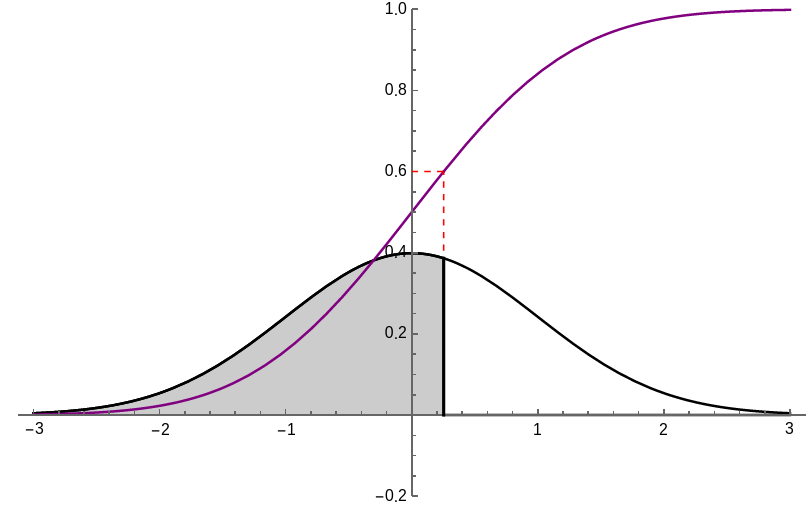
\includegraphics[scale = .25]{Images/PDF_CDF.png}
\caption{The density function $f(x)$ is the Bell-Shaped curve, the shaded are is $\mathbb{P}(X < .253) = \mathbb{P}(X \in (-\infty, .253)) = .60$. The function in the purple color is the cumulative distribution function (CDF) $F(x)$.}
\end{figure}

\item So the CDF or the cumulative distribution function $F(x)$ simply gives us the cumulative probabilities at each $x$.


\item  Once we understand what is cumulative probabilities, we can understand \alert{quantiles} or \alert{percentiles}.

\item In the last figure we showed


\begin{align*}
P ( X \leq 0.253) = F(0.253) = 0.6
\end{align*}

\item In this case we say the number $0.253$ is $0.6^{th}$ \alert{quantile} of the distribution. 

\item Notice this actually means $60\%$ values of the random variable is below $0.253$.

\item We also say $0.253$ is the $60^{th}$ \alert{percentile} of the distribution.

\item So quantiles and percentiles are same things, when it come to quantiles we write in decimals, for example $0.6$, $0.7$, etc. However for percentile we write $60\%$, $70\%$.

\item So if someone asks you what is $65\%$ percentile or $.65^{th}$ quantile of the distribution, you should say this is a value below which there are $65\%$ values of the random variable.




\end{itemize}
\end{frame}


\subsection{3. Summary Measures of a Distribution - Expectation $\mathbb{E}(\cdot)$ and Variance $\mathbb{V}(\cdot)$}

\frame{\subsectionpage}

\begin{frame}[allowframebreaks]{Continuous Probability Distributions}{Summary Measure - Expectation $\mathbb{E}(\cdot)$}

\begin{itemize}

\item Now let's see how to calculate the expected value of a continuous random variable $X$.



\begin{varblock}{\Thm{Definition } (Expectation)}

If $X$ is a continuous random variable with PDF $f(x)$, then the \alert{Expectation} of $X$ is defined as 

\begin{align*}
\mathbb{E}(X) =\int_{-\infty}^{\infty} x \; f(x) d x .
\end{align*}
	
\end{varblock}

\item We do it for the random variable we saw already, recall the PDF is given by,

\begin{align*}
f(x)= \begin{cases}2 x & \text { for } 0<x<1 \\ 0 & \text { otherwise. }\end{cases}
\end{align*}

\item We can calculate the expected value (just by \emph{replacing sum with integration!})

\begin{align*}
\mathbb{E}(X) &= \int_{-\infty}^{\infty} x f(x) d x = \int_{0}^{1} x (2x) dx = \int_{0}^{1} 2x^2 dx \quad \ldots \\	
\ldots &= 2 \int_{0}^{1} x^2 dx = 2 \times \left[\frac{x^2}{3}\right]^{^1}_{_{0}} = \frac{2}{3} \times \left[x^3\right]_{0}^{1}  \quad \ldots \\
\ldots &= \frac{2}{3} \times \left[{1^3} - {0^3}\right] = \frac{2}{3} \times 1 = \frac{2}{3} .
\end{align*}


\framebreak

\item Let's do another example. 

\item Let's calculate the expected value of the Uniform distribution where $X \sim \mathrm{Unif}(a, b)$

\begin{align*}
	\mathbb{E}(X) &= \int_{-\infty}^{\infty} x f(x) d x = \int_{a}^{b} x \frac{1}{b-a} dx = \frac{1}{b-a} \int_{a}^{b} x dx = \frac{1}{b-a} \left[\frac{x^2}{2}\right]_{a}^{b} \\
	&= \frac{1}{2(b-a)} \left[x^2\right]_{a}^{b} = \frac{1}{2(b-a)} \left[b^2 - a^2\right]  = \frac{b^2 - a^2}{2(b-a)} = \frac{(b+a)(b-a)}{2(b-a)} = \frac{b+a}{2}
\end{align*}


\item This means Expected value of a Uniformly distributed random variable is the average of the two end points of the interval. This seems very intuitive, since the probability is same for all values, so the expected value should be the average of the two end points. 

\item Question: What is the expected value of the random variable $X$ from the flight example? Recall $X \sim \mathrm{Unif}(60, 90)$



% \item \textbf{\color{red}A Notational Remark:}  You should always think about following picture if you think about Expectation of a random variable $X$. Often the constant that we get after calculating the expectation is denoted by $\mu$. So from now on, if you see $\mu$ (although sometimes this is a bit misleading because of normal random variable, we will see it later, but it's been used), you should understand this is an expected value like $1.5$.

% \begin{figure}
% 	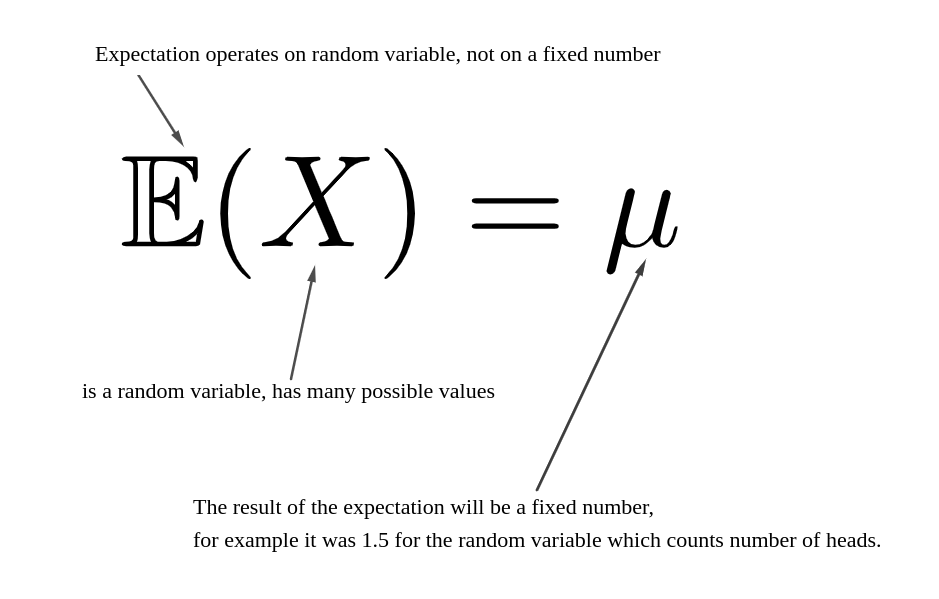
\includegraphics[scale = .3]{Images/Expectation_1.png}
% \end{figure}


% \item Finally always remember \alert{Population Mean, Expectation, Expected Value}, they are all same thing!




\end{itemize} 


\end{frame}



% \begin{frame}{Summary Measure - Expectation}

%  \begin{itemize}
%     \item So we get this expected value $1.5$, what does this mean?

%     \item Roughly you can interpret this like a \alert{central value} such that more probabilities (or weights) are near this value. This is why this is often called a measure for \alert{central tendency}!


%     \item Another name of Expectation is \alert{Population Mean}, or so often we will say \alert{Population Mean} rather than \alert{Expectation} (why Population?)

%     \item So \alert{Population Mean, Expectation, Expected Value}, they are all same thing!

%     \item Notice $1.5$ is between $1$ and $2$, and $1$ and $2$ are the two points where the probability is highest for this random variable.

%     \item Does this make sense? 


%     \item This is all about Expectation or Expected value of the random variable. 


%     \item Note that in this case, to calculate the Expected value we need to know the PMF (or all the probabilities when $X$ takes different values).


%     \item So if we don't know PMF then we cannot calculate expectation.

%     \item \textbf{\color{red}A notational remark:} Often the constant that we get after calculating the expectation is denoted by $\mu$. So from now on, if you see $\mu$, you should understand this is an expected value like $1.5$.

%     \item Now let's see about variance.

%   \end{itemize} 


% \end{frame}



\begin{frame}[allowframebreaks]{Continuous Probability Distributions}{Summary Measure - Variance $\mathbb{Var}\mathrm{ar}(\cdot)$}

\begin{itemize}
\item Like Expectation, variance is also a summary measure, where the expectation gives an idea of the central value, variance gives the idea how \alert{dispersed the values are}. 


\begin{varblock}{\Thm{Definition } (Variance)}

If $X$ is a continuous random variable with PDF $f(x)$, then the \alert{Variance} of $X$ is defined as 

\begin{align*}
\Var(X) = \mathbb{E}( (X-\mu)^2) =\int_{-\infty}^{\infty} (x-\mu)^2 f(x) d x .
\end{align*}
	
\end{varblock}

% \item First note that, Variance is also an Expectation, but it is an \alert{Expectation of $\left(X - \mu \right)^2$}, NOT $X$. 

% \item So what is $\left(X - \mu \right)^2$? Or what is $\left(X - \mu \right)$? Ans: $X - \mu$ is the deviation of the random variable from its Mean and $\left(X - \mu \right)^2$ is the squared deviation.

% \item So variance is the Expectation of the squared deviation.

% \item Let's calculate $\Var(X)$ for the random variable $X$, which counts the number of heads (PMF in page 27).

% \begin{align*}
% \Var(X) &= \left( \left(0 - 1.5\right)^2 \times f(0)\right) + \left( \left(1 - 1.5\right)^2 \times f(1)\right) + \\
% & \qquad \left( \left(2 - 1.5\right)^2 \times f(2)\right) + \left( \left(3 - 1.5\right)^2 \times f(3)\right) \\
% & = \left( \left(-1.5\right)^2 \times 1/8\right) + \left( \left(-0.5\right)^2 \times 3/8\right) + \left( \left(0.5\right)^2 \times 3/8\right) + \left( \left(1.5\right)^2 \times 1/8\right)\\
% &=\left(2.25 \times 1/8\right) + \left(0.25 \times 3/8\right) + \left(0.25 \times 3/8\right) + \left(2.25 \times 1/8\right) \\
% &= 0.75
% \end{align*}

% \item So calculating Variance is really easy, if we know PMF we can easily calculate the variance. 

% \item The interpretation of the variance is how dispersed the values are.

% \item \textbf{\color{red}A Notational remark:} Often the constant that we get after calculating the variance is denoted by $\sigma^2$. So from now on, if you see $\sigma^2$, you should understand this is a variance like $.75$.

% \item The square root of the variance is called \alert{Standard Deviation}, so if $\sigma^2$ is the Variance, then $\sigma$ is the standard deviation.



% \item Like discrete random variables we can also calculate Expected values and Variance for a continuous random variable.

\item The expectation and the variance of a continuous random variable can be calculated the same way we did for discrete, however, we need \alert{Integration} here (DIY \faEdit \faEdit \faEdit)



\end{itemize} 


\end{frame}


\section{Parametric Distributions : Continuous}
\frame{\sectionpage}

\subsection{1. Uniform Distribution}
\frame{\subsectionpage}

\begin{frame}[allowframebreaks]{Uniform Distribution}

\begin{itemize}

	\item Again we will see some parametric distributions, but now for continuous random variables. Recall \emph{parametric} means, there are one or two numbers in the PDF, that will specify the distributions, important is - \emph{knowing the parameters of the distribution means we know everything related to the distribution....}. We have already seen the details of the Uniform Distribution, so I won't repeat here,


	\item But here we give the definition again

	\framebreak


\begin{varblock}{Uniform Distribution}
A continuous random variable $X$ is said to follow the \alert{Uniform Distribution} on the interval $(a, b)$ if its PDF is

$$
f(x)= \begin{cases}\frac{1}{b-a} & \text { if } a<x<b, \\ 0 & \text { otherwise. }\end{cases}
$$

We denote this by $X \sim \operatorname{Unif}(a, b)$, where $a$ and $b$ are the parameters of the distribution and we have  

\begin{align*}
\mathbb{E}(X) &= \frac{a+b}{2} \\
\Var(X) &= \frac{(b-a)^2}{12}
\end{align*}

	
\end{varblock}

\medskip

\item Recall, we can also calculate 

		\begin{align*}
			\mathbb{P}(c < X < d) = \int_c^d f(x) \; dx =   \frac{1}{b-a} \times (d - c)
		\end{align*}




\end{itemize}
\end{frame}

\subsection{2. Normal Distribution}
\frame{\subsectionpage}


\begin{frame}[allowframebreaks]{Normal Distribution}

\begin{itemize}

\item Now we will see possibly one of the most important continuous probability distributions of all time.... that is \emph{Normal Distribution}



\begin{varblock}{Normal Distribution}
A continuous random variable $X$ is said to follow the \alert{Normal Distribution} with location parameter $\mu$ and dispersion parameter $\sigma^2$ if its PDF is

$$
f(x)= \frac{1}{\sqrt{2 \pi \sigma^2}} e^{-\frac{1}{2}\left(\frac{x-\mu}{\sigma}\right)^2}
$$

We denote this by $X \sim \mathcal{N}(\mu, \sigma^2)$, and we have  

\begin{align*}
\mathbb{E}(X) &= \mu \\
\Var(X) &= \sigma^2
\end{align*}

	
\end{varblock}

\framebreak

\item   When a random variable $X$ is normally distributed then we write $X \sim \mathcal{N}(\mu, \sigma^2)$. Here $\mu$ and $\sigma^2$ are the \alert{two parameters} of the distribution, which controls the shape of the density function $f(x)$. The density of the normal distribution looks like following.


\begin{figure}
\centering
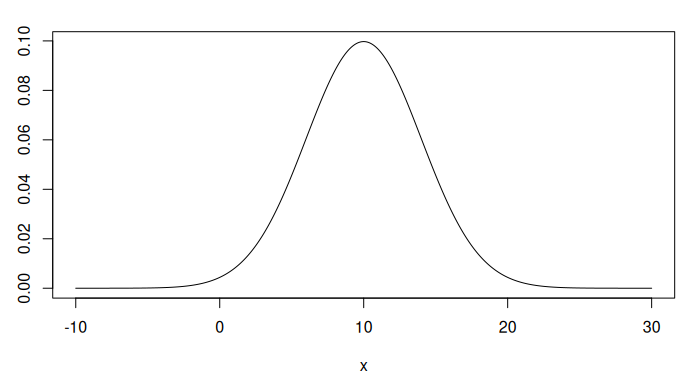
\includegraphics[scale = .4]{Images/pdfNormal_1.png}
\caption{density function of a normal distribution when $\mu = 10$ and $\sigma^2 = 16$}
\end{figure}

\item And the algebraic form of this function is

\begin{align*}
f\left(x\right)=\frac{1}{\sqrt{2 \pi \sigma^2}} e^{-\frac{1}{2}\left(\frac{x-\mu}{\sigma}\right)^2}
\end{align*}



\item Since we plotted the density in Figure 9 when $\mu = 10$ and $\sigma^2 = 16$, so this means the density function in Figure 8 is, 

\begin{align*}
f(x) = \frac{1}{\sqrt{2 \pi \times 16}} e^{-\frac{1}{2}\left(\frac{x-10}{4}\right)^2}
\end{align*} 


\item   The range of a normal distributed random variable is the whole real line or $\mathbb{R}$, so it takes values from $\infty$ to $+\infty$. 


\item $\mu$ is often called the \alert{location} parameter and $\sigma^2$ is called the \alert{dispersion} parameter, why this name?  This is because If we change $\mu$ and $\sigma^2$, then we can shift the location of the density and also change the spread of the density.... Following picture will help to understand this ...

\begin{figure}
\centering
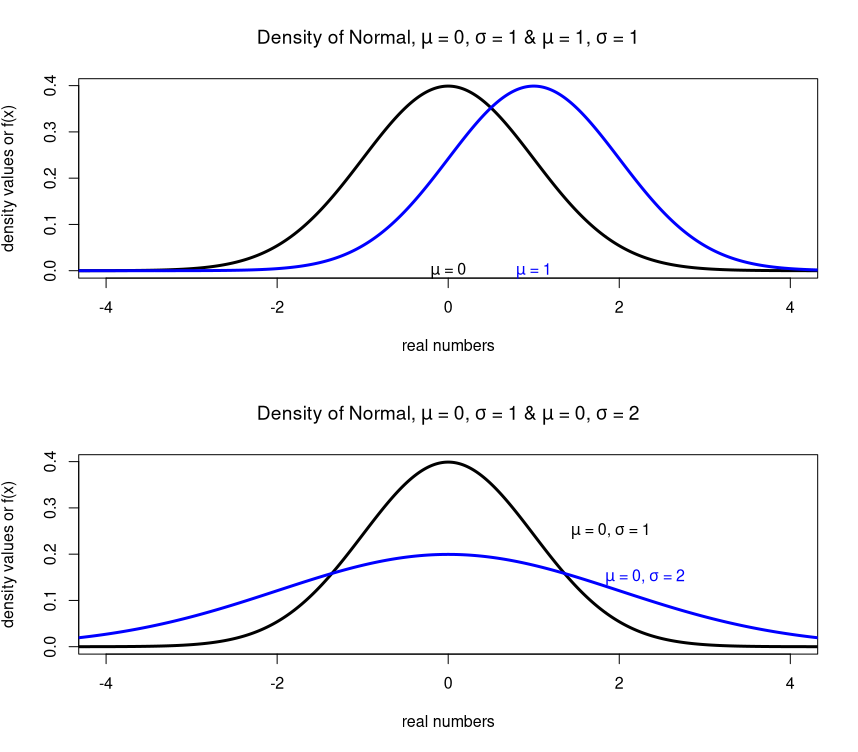
\includegraphics[scale = .3]{Images/Normal_density_parameter_change.png}
\caption{Effect of changing $\mu$ and $\sigma^2$ on the density function.}
\end{figure}

\item So for each combination of $\mu$ and $\sigma^2$, we will get a different density function. Recall we can use the density function to calculate different probabilities. So you should keep in mind - \emph{if parameters change then this means density changes and this then also means the probability distribution changes}.

\framebreak


\item For example, following is a density function with parameters $\mu = 0$, $\sigma^2 =1$, so the function is   $f(x) = \frac{1}{\sqrt{2 \pi}} e^{-\frac{1}{2}x^2}$. This normal distribution in particular is called \emph{Standard Normal Distribution}, so in this case $X \sim \mathcal{N}(0, 1)$

 

\begin{figure}
\centering
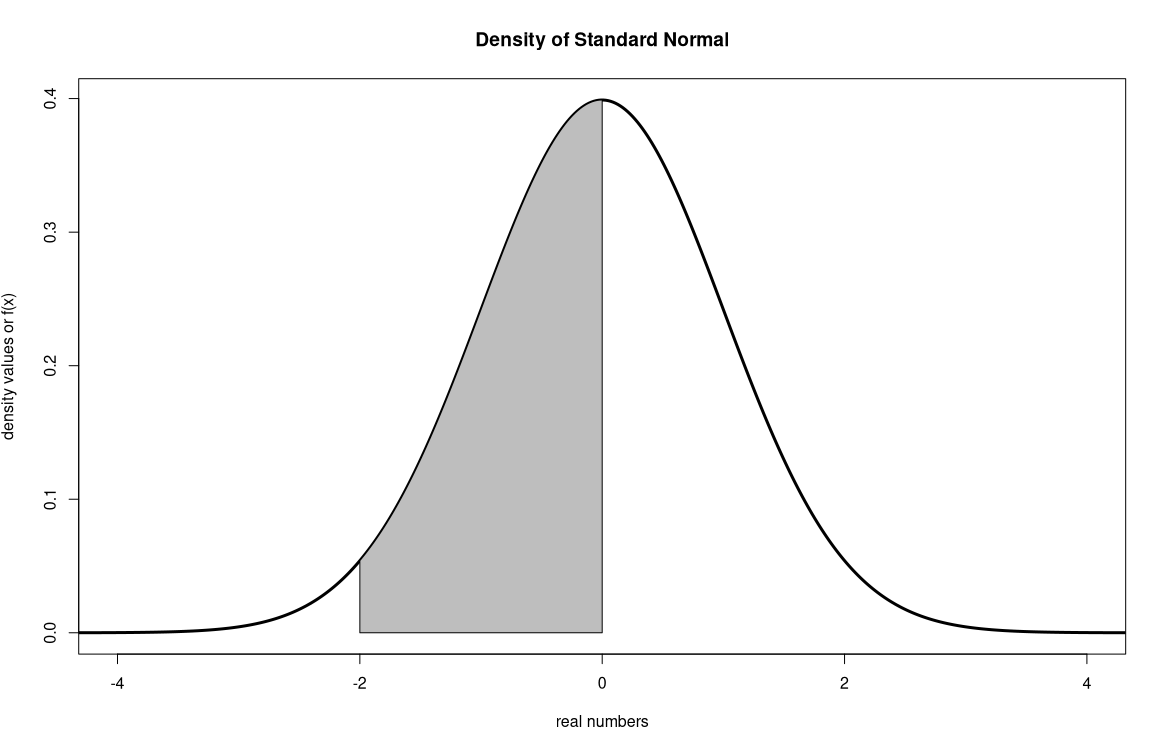
\includegraphics[scale = .25]{Images/Normal_density_area.png}
\caption{This is a density function for $X \sim \mathcal{N}(\mu, \sigma^2)$, so here $\mu = 0$, and $\sigma^2 = 1$. The shaded are is a probability, this is $\mathbb{P}(-2 < X < 0 )=\int_{-2}^0 f(x) d x=0.4772499$}
\end{figure}


\item We can use the density function to calculate the probabilities. Recall probability in this case is the area under the curve within some interval, right?

\item Notice for each combination of $\mu$ and $\sigma^2$, we will get a different density function, this means different probability distribution (why?)


\framebreak


\item Normal distribution has some amazing properties, even if you cannot remember the crazy looking density function, you should always remember these properties.

\framebrreak

\begin{varblock}{Some Properties of Normal Distribution}

\begin{itemize}
\item \textbf{Knowing Mean and Variance:} If $X \sim \mathcal{N}(\mu, \sigma^2)$ then,  $	\mathbb{E}(X) = \mu$ and $\Var(X) = \sigma^2$. Notice always in the figure the Mean (or expected value) $\mu$ will be at the center of the Normal distribution. 

\medskip

\item \textbf{3-$\sigma$ Rule:} You should also remember (look at the figure below, taken from Anderson)
%
\begin{align*}
	\mathbb{P}(\mu - \sigma < X < \mu + \sigma) &= 0.683 \\
	\mathbb{P}(\mu - 2\sigma < X < \mu + 2\sigma) &= 0.954 \\
	\mathbb{P}(\mu - 3\sigma < X < \mu + 3\sigma) &= 0.997
\end{align*}

% \begin{itemize}
% \item   the two points $\mu + \sigma$,  $\mu - \sigma$, and we know that within these two points there will be $68.3\%$ probability. 
% \item   the two points $\mu + 2\sigma$,  $\mu - 2\sigma$, and we know that within these two points there will be $95.4\%$ probability. 
% \item   the two points $\mu + 3\sigma$,  $\mu - 3\sigma$, and we know that within these two points there will be $99.7\%$ probability. 

% \end{itemize}

\item \textbf{Standardization Rule:} Finally if we know the random variable $X \sim \mathcal{N}(\mu, \sigma^2)$, then we can \emph{transform} $X$ to $Z$ (or standardize) with
%
\begin{align*}
Z = \frac{X - \mu}{\sigma}
\end{align*}

where $Z \sim \mathcal{N}(0, 1)$ (It's also possible to go from $Z$ to $X$ if you know $\mu$ and $\sigma^2$)

\medskip

\end{itemize}

\end{varblock}

\framebreak

\item First property is obvious...


\item For the second property, look at the picture below,

\begin{figure}[H]
\centering
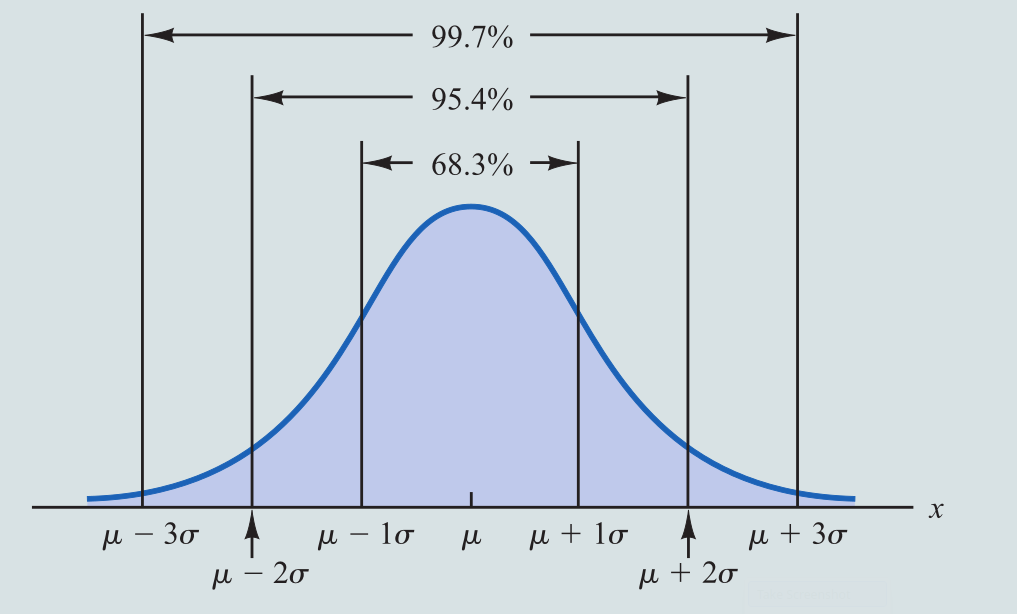
\includegraphics[scale = .25]{Images/PDF_Normal_percentiles.png}
\caption{Picture taken from \cite{anderson_statistics_2020}, this is called the famous $3-\sigma$ rule, which says $68.3\%$, $95.4\%$ and $99.7\%$ of the values are within $1$, $2$ and $3$ standard deviations from the mean $\mu$.}
\end{figure}



\item This means if we know the mean $\mu$ and variance $\sigma^2$, then we can figure out certain probabilities

\framebreak




\item The last property is what we call \alert{$Z$-transformation, or standardization or normalization}. All it says is - 

\medskip

\emph{if we have a normal random variable with mean $\mu$ and variance $\sigma^2$, then we can transform this and get a standard normal random variable with mean $0$ and variance $1$. Here transformation means taking each of the values and then subtracting the mean $\mu$ and dividing by the standard deviation $\sigma$. This is also called \alert{standardization}}.


\item This is a very useful rule because we can go back and forth from $\mathcal{N}(\mu, \sigma^2)$ to $\mathcal{N}(0, 1)$. In the back of your book you have a table of Standard Normal Distribution, we will do some problems then you will understand why this is useful. 




\item I think now we are ready to do some problems in \cite{anderson_statistics_2020}, we will use the standard normal table at the back of the book 




\framebreak



\item \textbf{An Interesting point}: Interestingly we can do the standardization for sample data coming from any distribution, not necessary normal... so from $x_1, \ldots. x_n$,  calculate

\begin{align*}
\bar{x} = \frac{1}{n} \sum_{i=1}^{n} x_i, \quad s^2_x = \frac{1}{n} \sum_{i=1}^{n} (x_i - \bar{x})^2
\end{align*}

and then we can calculate the standardized value for $x_i$ as

\begin{align*}
z_i = \frac{x_i - \bar{x}}{s_x}
\end{align*}

where $z_i$ is the standardized value for $x_i$, then we will also get 

\begin{align*}
\bar{z} = \frac{1}{n} \sum_{i=1}^{n} z_i = 0 \quad s^2_z = \frac{1}{n} \sum_{i=1}^{n} (z_i - \bar{z})^2 = 1
\end{align*}



\end{itemize}


\end{frame}




% % \begin{frame}{Distribution, Mean and Variance}

% % \begin{itemize}

% % \item Before we proceed further let's summarize what we did so far.

% % \item So we had a discrete random variable $X$ which takes values $0, 1, 2, 3$ and it has following PMF,

% % \vspace*{-.3cm}
% % \begin{align}
% % f(x)= \begin{cases} 1/8 & \text { if } x=0 \\ 
% % 3/8 & \text { if } x=1 \\ 
% % 3/8 & \text { if } x=2 \\ 
% % 1/8 & \text { if } x=3 \\ 
% % 0 & \text { otherwise }\end{cases}
% % \end{align}

% % \item PMF tells us about the distribution, because it tells about $\mathbb{P}(X = 0), \mathbb{P}(X = 1), \mathbb{P}(X = 2)$ and $\mathbb{P}(X = 3)$.

% % \item But distribution is often too much information, and maybe sometimes we just one or two numbers to understand about the distribution of a random variable. This is what the job of Mean and Variance of the distribution.

% % \item Where Mean of the distribution gives us an idea about the central point, the Variance tells us how spread the distribution is, and Standard deviation is just the square root of the Variance.

% % \item For this random variable $\mathbb{E}(X) = 1.5$ and $\Var(X) = .75$, and standard deviation is $\sqrt{.75}$.



% % \end{itemize} 


% % \end{frame}


% \section{Parametric Family of Probability Distributions}
% \frame{\sectionpage}


% \subsection{Discrete Distribution - Bernoulli and Binomial Distribution}
% \frame{\subsectionpage}



% \begin{frame}[allowframebreaks]{Bernoulli \& Binomial Random Variables}





% \begin{itemize}

% \item If a random variable $X$ has only two values $0$ and $1$, we call the random variable a \alert{Bernoulli Random variable}, and its distribution is known as \alert{Bernoulli distribution},  some examples, 

% \begin{itemize}
% \item Random Experiment - Toss a coin. Random Variable $X = 1$ means head, $X = 0$ means tail.

% \item Random Experiment - Pick a random person from a Population of people. Random Variable $X = 1$ means female, and $X = 0$ means male 

% \item Random Experiment - Calling a customer.  Random Variable $X = 1$ means picked up the call, $X = 0$ means didn't pickup.

% \end{itemize}

% \item In practice or in real life scenario, when you have possible data with $0, 1, 0, 1, 0, 1$, you can think about these are values of some Bernoulli random variables. So in any experiment, when we have only two possible outcomes we can think about a modeling that experiment using a Bernoulli random variable. For a Bernoulli random variable, if $X = 1$, we often call it \emph{``success''} and if $X = 0$, we often call it ``failure''. Here is the formal definition.

% \begin{varblock}{\Thm{Definition } (Bernoulli Distribution)}
%  \Thm{Definition } (Bernoulli distribution). A random variable $X$ is said to have the Bernoulli distribution with parameter $p$ (we wrote $X \sim \operatorname{Bernoulli}(p)$), if $\mathbb{P}(X=1)= p$ and $\mathbb{P}(X=0)= 1-p$. The PMF of $X$ can be written as,

% \begin{align*}
% f(x; p) &= p^x {(1 - p)}^{1-x}, \quad \text{ when } x = 0, 1 \\
% &  = 0, \quad \text{otherwise}
% \end{align*}

% where $0<p<1$
% \end{varblock}



% \item Note that, because of this PMF, we have $\mathbb{P}(X=1)=f(1) = p$ and $\mathbb{P}(X=0)= f(0) = 1-p$.

% \item Notice, the parameter $p$ controls the probability and hence controls the distribution of the random variable. For example, if $X \sim \operatorname{Bernoulli}(.3)$, this automatically means $\mathbb{P}(X = 1) = 0.3$ and $\mathbb{P}(X = 0) = 0.7$. Here is how the PMF will look like for different parameters $p$,

% \begin{figure}
% 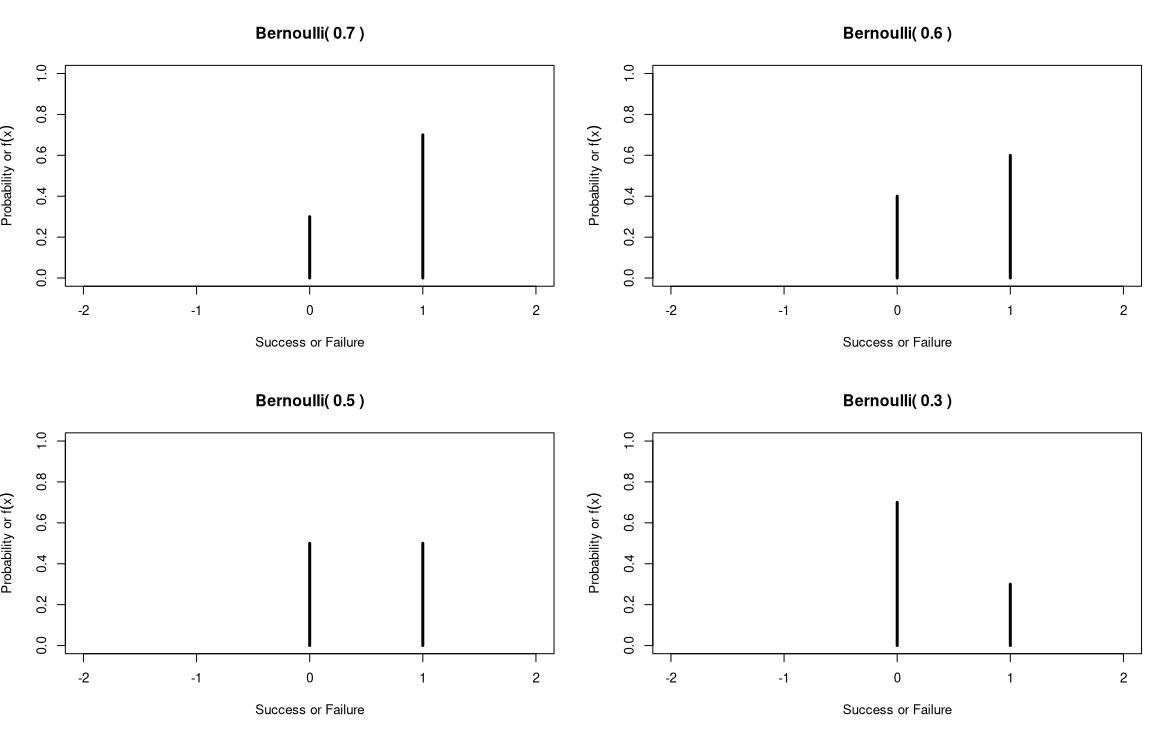
\includegraphics[scale = .3]{Images/BernoulliDistPMF.png}
% \end{figure}


% \item Because we have the PMF we can also calculate the Expected Value and Variance of a Bernoulli random variable.

% \item If you do the calculation, then you should get $\mathbb{E}(X) = p$ and $\Var(X) = p (1-p)$ (please do the calculation!)

% \framebreak

% \item The Binomial distribution comes when we perform \emph{$n$ independent Bernoulli experiment}.

% \item Here is the story - Suppose now we perform $n$ independent Bernoulli experiments (or Bernoulli trials) with parameter $p$. If $X$ is a random variable which represents the total number of success out of the $n$ trials, then we say the random variable $X$ follows Binomial distribution with parameter $n$ and $p$.

% \item You already know the example, if we toss a single coin and represent $X$ as a Bernoulli random variable which can take values $1$ (success) or $0$ (failure) with probability $p$, then when we toss $n = 3$ independent coins and represent $X$ as total number of heads (total number of success), then $X$ is said to follow Binomial with parameter $n = 3$ and probability $p$.


% \begin{varblock}{\Thm{Definition } (Binomial Distribution)}
% 	Suppose that $n$ independent Bernoulli trials are performed, each with the same success probability $p$. Let $X$ be the number of successes. The distribution of $X$ is called the Binomial distribution with parameters $n$ and $p$. We write $X \sim \operatorname{Bin}(n, p)$ to mean that $X$ has the Binomial distribution with parameters $n$ and $p$, where $n$ is a positive integer and $0<p<1$. The PMF of $X$ can be written as 

% \begin{align*}
% f(x; n, p)&=\left(\begin{array}{l}
% n \\
% x
% \end{array}\right) p^x(1-p)^{n-x} \quad \text{ for } x = 0, 1, 2, \ldots, n \\
% &= 0, \text{ otherwise}
% \end{align*}
% \end{varblock}


% \item Notice here $x$ is the value of the random variable where $x$ can be $0, 1, 2, \ldots, n$. The PMF looks very similar to Bernoulli PMF, except we have a combination term, recall $\left(\begin{array}{l}
% n \\
% x
% \end{array}\right) = \Combine[n]{x} = \frac{n!}{x! (n-x)!}$. Question is why is this coming? 


% \item Here is a short answer, the experiment consisting of $n$ independent Bernoulli trials produces a sequence of successes and failures. The probability of any specific sequence of $x$ successes and $n-x$ failures is $p^x(1-p)^{n-x}$. There are $\Combine[n]{x}$ such sequences.



% \item We can also calculate the Mean and the Variance of the Binomial distribution. \alert{If $X \sim \textrm{Bin}(n, p)$, then $\mathbb{E}(X) = np$ and $\Var(X) = np(1-p)$}, where do we get this? You can see the proof in the next page. However there is an easy trick that is you remember Binomial is the sum $n$ independent Bernoulli trials (Let's do it using easy trick!)

% \framebreak


% \item If $X \sim \mathrm{Bin}(n, p)$, then applying the formula for Expectation

% $$
% \mathbb{E}(X)=\sum_{x=0}^n x f(x)=\sum_{x=0}^n x\left(\begin{array}{l}
% n \\
% x
% \end{array}\right) p^x q^{n-x} .
% $$

% \item Note here we wrote $q = (1-p)$. Also note that we have $x\left(\begin{array}{c}n \\ x\end{array}\right)=n\left(\begin{array}{c}n-1 \\ x-1\end{array}\right)$, so
% $$
% \begin{aligned}
% \sum_{x=0}^n x\left(\begin{array}{l}
% n \\
% x
% \end{array}\right) p^x q^{n-x} &=n \sum_{x=0}^n\left(\begin{array}{c}
% n-1 \\
% x-1
% \end{array}\right) p^x q^{n-x} \\
% &=n p \sum_{x=1}^n\left(\begin{array}{c}
% n-1 \\
% x-1
% \end{array}\right) p^{x-1} q^{n-x} \\
% &=n p \sum_{j=0}^{n-1}\left(\begin{array}{c}
% n-1 \\
% j
% \end{array}\right) p^j q^{n-1-j} \\
% &=n p .
% \end{aligned}
% $$

% Then \emph{we get $\mathbb{E}(X) = np$, similarly we can derive the variance is $\mathbb{V}\mathrm{ar}(X) = np(1-p)$ (I am skipping the proof). Again the easy trick is to apply Binomial - Bernoulli relation}.


% \item Here is how the PMF will look like for two Binomial distributions, with same $n = 3$ but different $p$.

% \begin{figure}
% 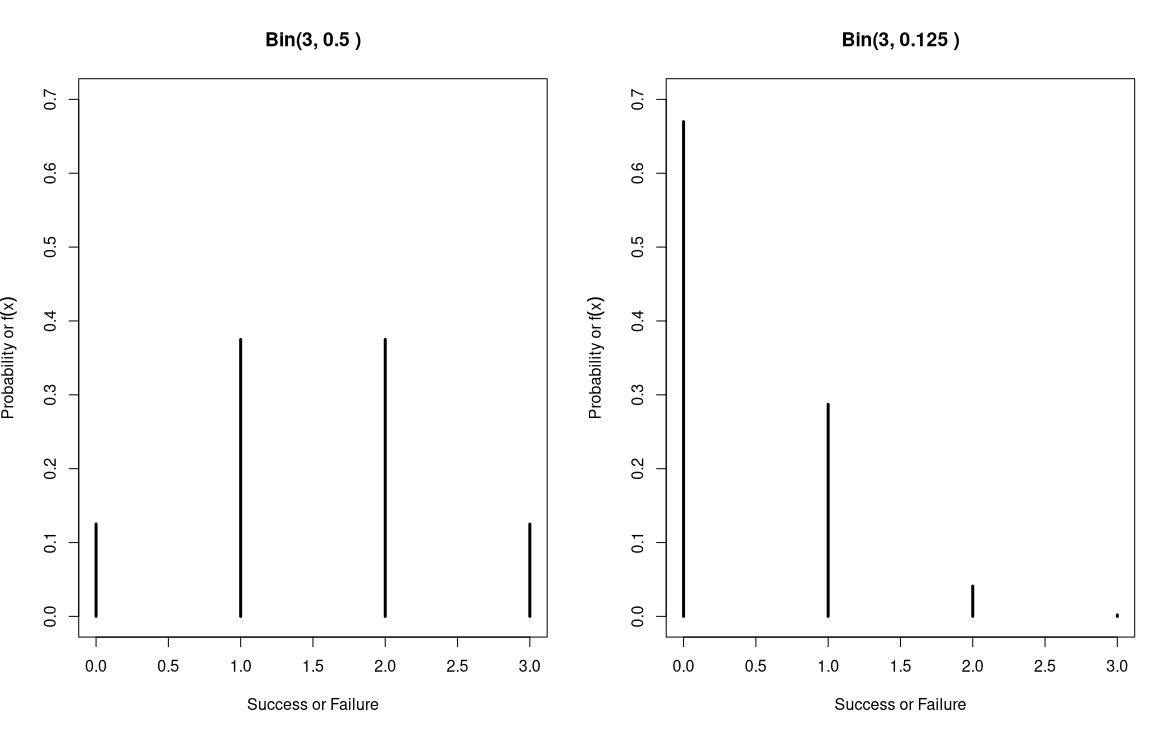
\includegraphics[scale = .3]{Images/Binomial-1.png}
% \caption{On the left we have the PMF of $X \sim \textrm{Bin}(3, 0.5)$ and on the right we have $X \sim \textrm{Bin}(3, 0.125)$.  }
% \end{figure}



% \begin{figure}
% 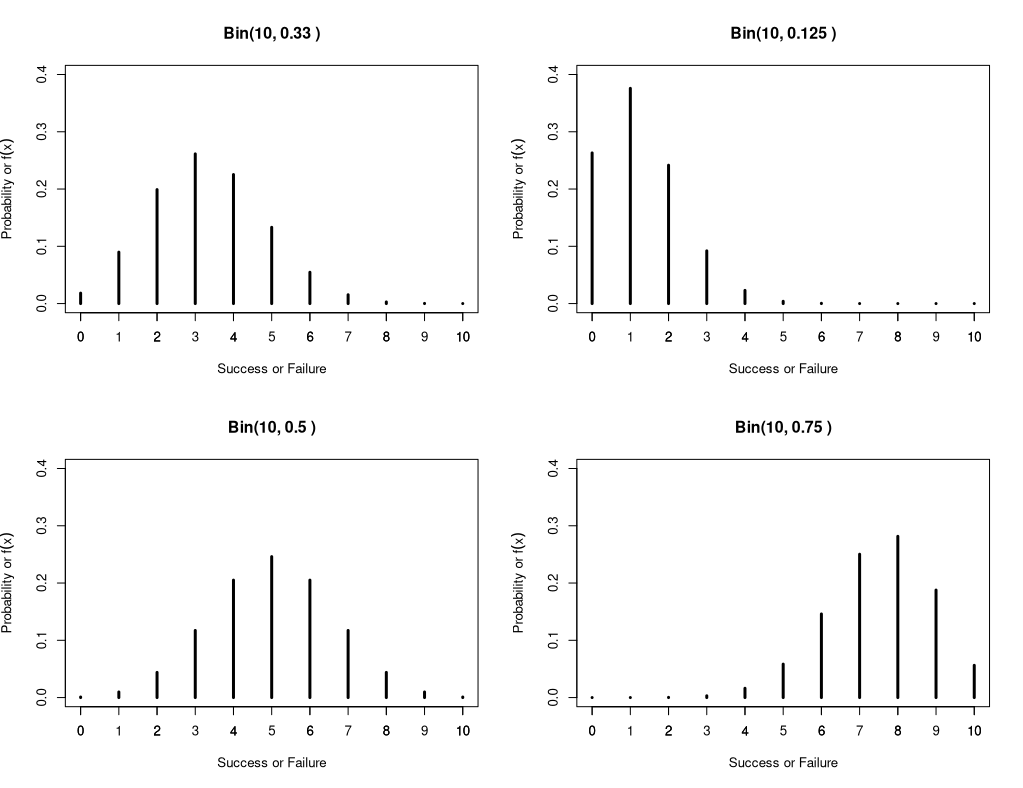
\includegraphics[scale = .3]{Images/Binomial-2.png}
% \caption{From top left, we have the PMF of $X \sim \textrm{Bin}(10, 0.33)$, then right $X \sim \textrm{Bin}(10, 0.125)$, then bottom left $X \sim \textrm{Bin}(10, 0.5)$ and right $X \sim \textrm{Bin}(10, 0.75)$  }
% \end{figure}


% \item Binomial distribution comes in many forms in real life, you should always remember the essential structure - \emph{that is tossing $n$ independent coins and then the random variable is the number of success out of $n$}.

% \item Here are some examples where we can think about a Binomial random variable.

% \begin{itemize}
% \item  Random experiment: Calling $n$ people. Random variable $X$ will represent how many people will answer the call.

% \item Random experiment: $n$ students registered for a course. Random variable $X$ will represent how many students will finish it.

% \item Random experiment: Randomly asking $5$ people whether they are satisfied with the transportation system of Bangladesh. Random variable is number of people who said "yes"! 

% \item And there are more examples in \cite{anderson_statistics_2020}.


% \end{itemize}

% \item Notice two important assumptions for the Binomial random variable is, 1) all trials are independent and 2) all trials happens with same probability. Only in these cases you can think about the random variable is Binomial.



% \end{itemize}


% \end{frame}



% \subsection{Discrete Distribution - Poisson Distribution}
% \frame{\subsectionpage}



% \begin{frame}[allowframebreaks]{Poisson Distribution}


% \begin{itemize}
% \item Now we will consider another distribution known as Poisson distribution. 

% \item The situation when you can use Poisson distribution is very similar to Binomial distribution, but the difference is in Binomial you have often a small number of trials, but in Poisson you may have many (in theory infinite) independent trials, with success probability very small.

% \item For example, the number of arrivals at a car wash in one hour, the number
% of repairs needed in 10 miles of highway, or the number of leaks in 100 miles of pipeline (these examples are from \citet*{anderson_statistics_2020}). Notice, $n$ can be very large, often there is no upper limit, and also the values $x$ also has no upper limit, so it can be $0, 1, 2, 3, \ldots$.


% \begin{varblock}{\Thm{Definition } (Poisson Distribution)}
% An random variable $X$ has the Poisson distribution with parameter $\lambda$ if the $\mathrm{PMF}$ of $X$ is

% \begin{align*}
% f(x; \lambda) = \frac{e^{-\lambda} \lambda^x}{x !}, \quad x=0,1,2, \ldots
% \end{align*}


% We write this as $X \sim \operatorname{Pois}(\lambda)$.	
% \end{varblock}


% \item This is a valid PMF because we can show that $\sum_{x=0}^{\infty} \frac{\lambda^x}{x !}=e^{\lambda}$.

% \framebreak

% \item How does Poisson PMF come? The idea is we can think Poisson distribution is a \emph{limiting case} (or limit) of Binomial distribution. More specifically we need $n \to \infty$ and $p \to 0$, then Binomial PMF will converge to Poisson PMF.

% \item This means starting from $    \left(\begin{array}{l}
% n \\
% x
% \end{array}\right) p^x(1-p)^{n-x}$ and we take   $n \to \infty$  and $p \to 0$  we get  $\frac{e^{-\lambda} \lambda^x}{x !}$


% \item It's a mathematical problem with limit, so we will avoid it, but you should understand that Poisson distribution appears as a limit of Binomial.

% \framebreak

% \item In real life context it  is often used in situations where we are counting the number of successes in a particular region or interval of time, and there are a large number of trials, each with a small probability of success. The random variable $X$ is again the number of success and but in this case number of success can be $0, 1, 2, 3, \ldots $.

% \item Here are some more examples, 

% \begin{itemize}
% 	\item The number of emails you receive in an hour. There are a lot of people who could potentially email you in that hour, but it is unlikely that any specific person will actually email you in that hour.

% 	\item The number of earthquakes in a year in some region of the world. At any given time and location, the probability of an earthquake is small, but there are a large number of possible times and locations for earthquakes to occur over the course of the year. 

% \end{itemize}


% \item There are more example in \cite{anderson_statistics_2020}.

% \item If $X \sim \mathrm{Pois}(\lambda)$, then we can again calculate (skip the proof)

% \begin{align*}
% \mathbb{E}(X) = \lambda \quad \text{ and } \quad \Var(X) = \lambda
% \end{align*}



% \item Here $\lambda$ is the parameter, which is also the mean or expected value. It is often it is called the \emph{rate of occurrence} in the rare events.


% \framebreak

% \item There are other discrete distributions, e.g., Geometric and Negative Binomial, which we won't cover here. If you are interested to read about them you can read \cite{degroot_probability_2012}.

% \end{itemize}


% \end{frame}

% \subsection{Continuous Distribution - Normal Distribution}
% \frame{\subsectionpage}


% \begin{frame}[allowframebreaks]{Normal Distribution}

% \begin{itemize}

% \item We already saw one continuous distribution, which is Uniform distribution, now we will see another one, known as \alert{Normal distribution}.

% \item \alert{Normal distribution} is possibly one of the most important continuous probability distributions of all time.

% \item   When a random variable $X$ is normally distributed then we write $X \sim \mathcal{N}(\mu, \sigma^2)$. Here $\mu$ and $\sigma^2$ are the \alert{two parameters} of the distribution, which controls the shape of the density function $f(x)$. The density of the normal distribution looks like following.


% \begin{figure}
% \centering
% 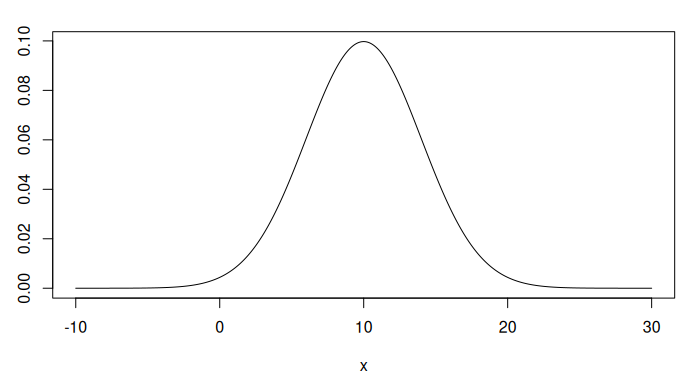
\includegraphics[scale = .4]{Images/pdfNormal_1.png}
% \caption{density function of a normal distribution when $\mu = 10$ and $\sigma^2 = 16$}
% \end{figure}

% \item What is the algebraic form of this function? Here it is

% \begin{align*}
% f\left(x ; \mu, \sigma^2\right)=\frac{1}{\sqrt{2 \pi \sigma^2}} e^{-\frac{1}{2}\left(\frac{x-\mu}{\sigma}\right)^2}
% \end{align*}



% \item Since we plotted the density in Figure 10 when $\mu = 10$ and $\sigma^2 = 16$, so this means the density function in Figure 8 is, 

% \begin{align*}
% f(x; 10, 16) = \frac{1}{\sqrt{2 \pi \times 16}} e^{-\frac{1}{2}\left(\frac{x-10}{4}\right)^2}
% \end{align*} 


% \item   The range of a normal distributed random variable is the whole real line or $\mathbb{R}$. This means it takes values from $\infty$ to $+\infty$. 


% \item $\mu$ is often called the \alert{location} parameter and $\sigma^2$ is called the \alert{dispersion} parameter (why this name, we will see in a minute)


% \item Again notice this is a function of $x$, but we also wrote the two parameters $\mu, \sigma^2$ after ``$;$'', always remember when we think about a density function now it's a function of $x$ (this is similar to PMF) but we will write parameters to show that these parameters controls the function. 


% \item We can use the density function to calculate the probabilities. Recall probability in this case is the area under the curve within some interval, right?

% \item For example, following is a density function with parameters $\mu = 0$, $\sigma^2 =1$, so the function is   $f(x; 0, 1) = \frac{1}{\sqrt{2 \pi}} e^{-\frac{1}{2}x^2}$.


% \begin{figure}
% \centering
% 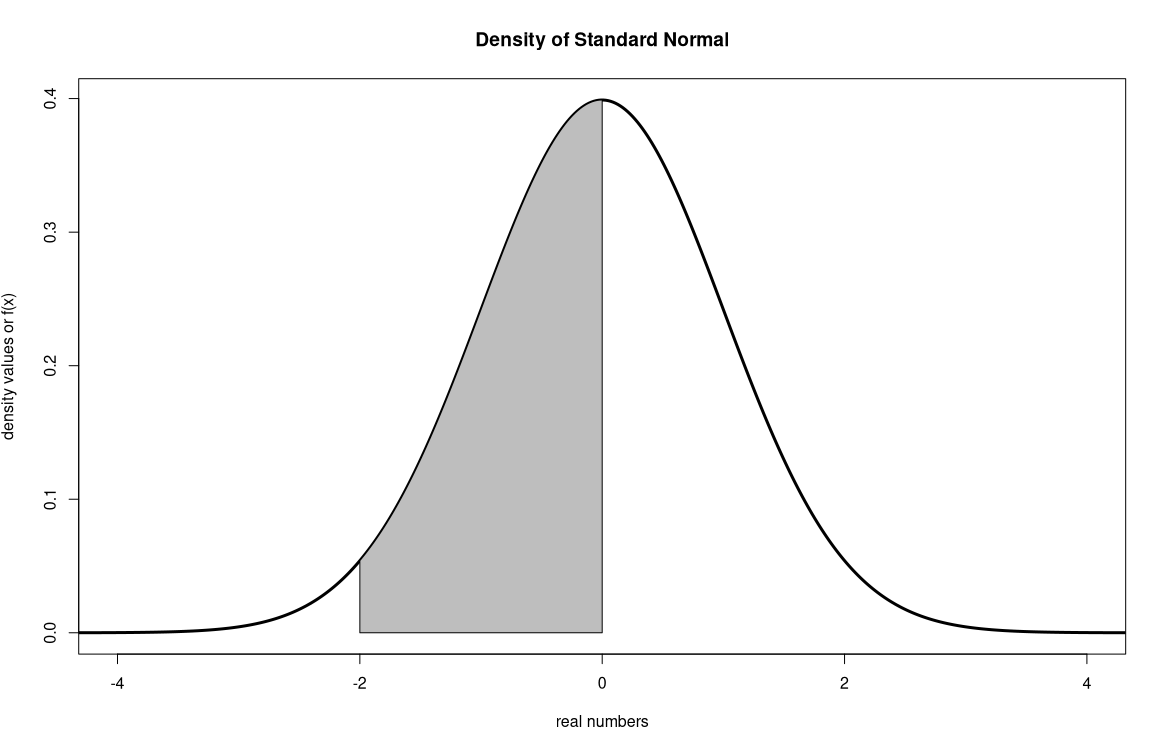
\includegraphics[scale = .25]{Images/Normal_density_area.png}
% \caption{This is a density function of a normal distribution with $\mu = 0$, and $\sigma^2 = 1$. The shaded are is a probability, this is $\mathbb{P}(X \in(-2,0))=\int_{-2}^0 f(x; 0, 1) d x=0.4772499$}
% \end{figure}




% \item Notice for each combination of $\mu$ and $\sigma^2$, we will get a different density function, this means different probability distribution (why?.

% \item Why we call them \alert{location} and \alert{dispersion} parameter. This is because If we change $\mu$ and $\sigma^2$, then we can shift the location of the density and also change the spread of the density.

% \begin{figure}
% \centering
% 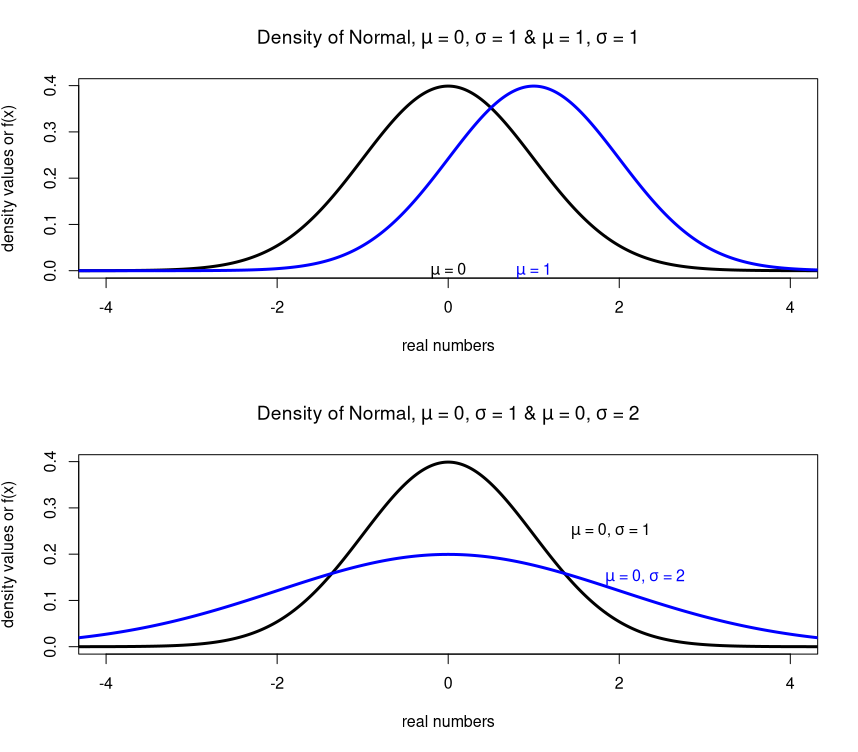
\includegraphics[scale = .3]{Images/Normal_density_parameter_change.png}
% \caption{Effect of changing $\mu$ and $\sigma^2$ on the density function.}
% \end{figure}

% \item So for each combination of $\mu$ and $\sigma^2$, we will get a different density function. Recall we use the density function to calculate different probabilities. So density change is equivalent to distribution change.

% \framebreak


% \item Normal distribution has some amazing properties, even if you cannot remember the crazy looking density function, you should always remember these properties.

% \begin{itemize}
% \item If $X \sim \mathcal{N}(\mu, \sigma^2)$ We can calculate the Expected value and Variance. We will get $\mathbb{E}(X) = \mu$ and $\Var(X) = \sigma^2$.

% \item Notice the figure the Mean (or expected value) will be always at the center of the Normal distribution. 

% \item Then you should remember following picture (this is taken from \cite{anderson_statistics_2020})
% \medskip

% \end{itemize}

% \item[]

% \begin{itemize}
% \item[]

% \begin{figure}
% \centering
% 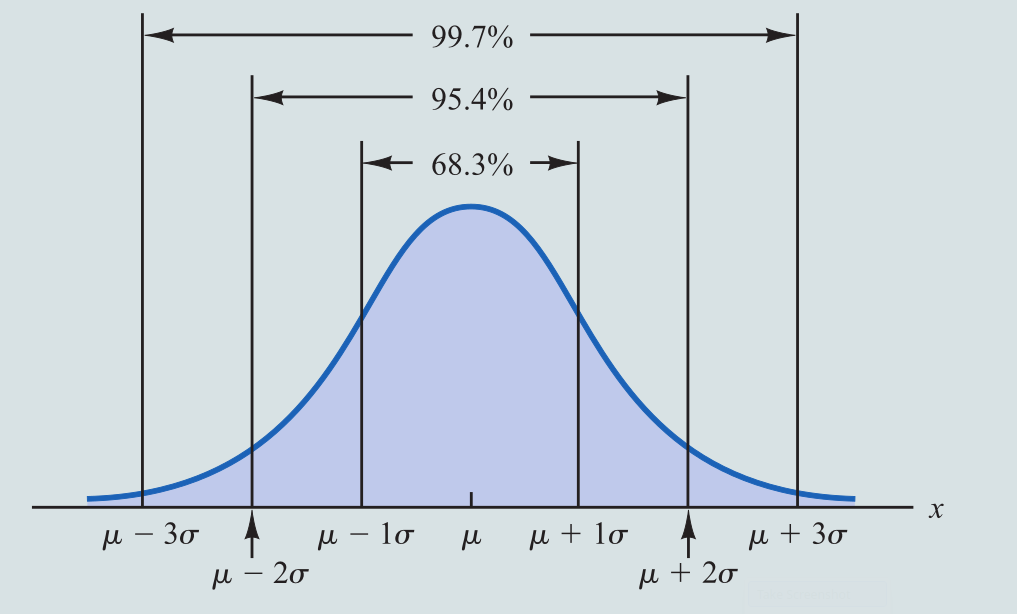
\includegraphics[scale = .25]{Images/PDF_Normal_percentiles.png}

% \end{figure}
% \end{itemize}

% \item This means if we know the mean $\mu$ and variance $\sigma^2$, then we can figure out 

% \begin{itemize}
% \item   the two points $\mu + \sigma$,  $\mu - \sigma$, and we know that within these two points there will be $68.3\%$ probability. 
% \item   the two points $\mu + 2\sigma$,  $\mu - 2\sigma$, and we know that within these two points there will be $95.4\%$ probability. 
% \item   the two points $\mu + 3\sigma$,  $\mu - 3\sigma$, and we know that within these two points there will be $99.7\%$ probability. 

% \end{itemize}



% \item Finally if we know the random variable $X \sim \mathcal{N}(\mu, \sigma^2)$, then we can transform this random variable and get a new random variable $Z$, by

% \begin{align*}
% Z = \frac{X - \mu}{\sigma}
% \end{align*}

% \item This what we call \alert{$Z$-transformation, or standardization or normalization}.

% \item The interesting thing is it can be proven that $Z \sim \mathcal{N}(0, 1)$.

% \item This is sometimes very helpful because we can go back and forth from $\mathcal{N}(\mu, \sigma^2)$ to $\mathcal{N}(0, 1)$.


% \item I think now we are ready to do some problems in \cite{anderson_statistics_2020}, we will use the standard normal table at the back of the book 

% \end{itemize}


% \end{frame}




% \subsection{Continuous Distribution - Exponential Distribution}
% \frame{\subsectionpage}


% \begin{frame}{Exponential Distribution}



% \end{frame}


% \section{Rules of Expectation and Variance}
% \frame{\sectionpage}


% \begin{frame}[allowframebreaks]{Rules of Expectation and Variance}

% \begin{itemize}
% \item We already saw the way to calculate the Expected value\footnote[frame]{Recall we call it also mean or expectation.} of a random variable $\mathbb{E}(X)$, when $X$ is discrete or continuous. Here are the two formulas again

% \begin{align*}
% \mathbb{E}(X) &= \sum_{\text {all values } x} x f(x) \quad \text{ [when $X$ is discrete]}\\
% \mathbb{E}(X) &=\int_{-\infty}^{\infty} x f(x) d x \quad \text{ [when $X$ is continuous]} 
% \end{align*}


% \item The Variance is also an expectation, but it's the expectation of the squared deviation from mean.

% \vspace*{-.3cm}
% \begin{align*}
% \Var(X) &= \mathbb{E} \left(  \left( X - \mathbb{E}(X) \right)^2 \right)=  \sum_{\text {all values } x} (x - \mathbb{E}(X) )^2  f(x) \quad \text{ [when $X$ is discrete]} \\
% \Var(X) &= \mathbb{E} \left(  \left( X - \mathbb{E}(X) \right)^2 \right)= \int_{-\infty}^{\infty}  (x - \mathbb{E}(X) )^2  f(x) dx  \quad \text{ [when $X$ is continuous]}
% \end{align*}

% \item Always remember! The expected value of a random variable is a constant, so $\mathbb{E}(X) = \text{ constant number }$. Sometimes we write this constant number with $\mu$ regardless of the fact that $X$ follows normal distribution or not. This is not a good notation, but people generally use it.

% \bigskip

% \item Again you should always keep the following picture in your mind, that expectation works on random variables, not on number, and the result of Expectation is a constant.


% \begin{figure}
% 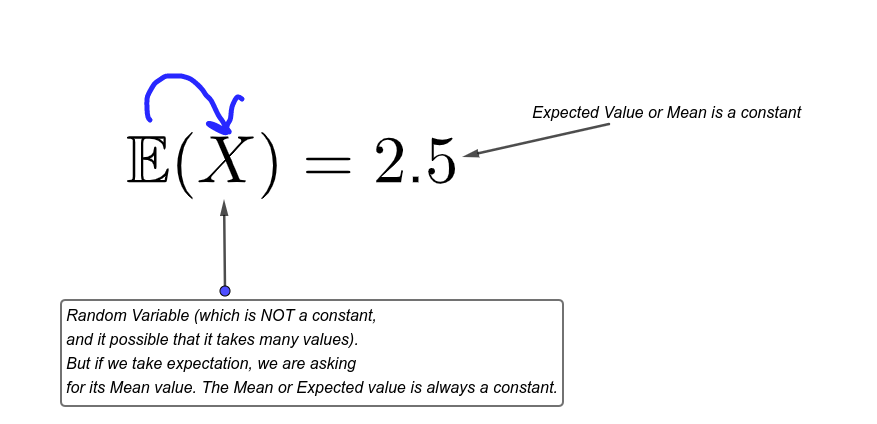
\includegraphics[scale = .5]{Images/RV_1.png}
% \end{figure}




% \item Now we consider a slightly different problem, we ask what is 

% {\huge{
% \vspace*{-.5cm}
% \begin{align*}
% \mathbb{E}(X^2) \text{ or } \mathbb{E}(X^3)  \text{ or } \mathbb{E}(2X + 3) \text{ ??? }
% \end{align*}
% }}

% \item Note that $X^2$, $X^3$ or $2X + 3$ are all functions of random variable $X$. 

% \item So our question is for a function $g(X)$, where $g(X)$ can be $X^2$, $X^3$ or $2X + 3$, what is $\mathbb{E}(g(X))$?

% \item First of all note that $g(X)$ is also a random variable. So a function of a random variable is also a random variable.

% \item It turns out that (we are avoiding the formal proof) in this case we can calculate $\mathbb{E}(g(X))$ by using the distribution of $X$. 

% \item So this means ....

% \begin{align*}
% \mathbb{E}(g(X)) &= \sum_{\text {all values } x} g(x) f(x) \quad \text{ [when $X$ is discrete]}\\
% \mathbb{E}(g(X)) &=\int_{-\infty}^{\infty} g(x) f(x) d x \quad \text{ [when $X$ is continuous]} 
% \end{align*}

% \item Now we can apply this rule more or less for any function $g()$. This rule has an interesting name, it is called - \alert{Law of the unconscious Statistician} or in short \alert{LOTUS} (why this name?)

% \item We have already applied LOTUS previously,

% \begin{itemize}
% \item Calculating variance is an application of this rule, because we are doing $\mathbb{E}\left( \left( X - \mu  \right)^2  \right)$. Here $g(X) =  \left( X - \mu  \right)^2 $.

% \item Also in PS-3 when we calculated $\mathbb{E}\left( X^2  \right)$, we have applied LOTUS, here $g(X) = X^2$.

% \item You can create more examples, but application of LOTUS is easy!
% \end{itemize}

% \item So LOTUS is one rule for expectation, there are two other rules for expectation, and we can use LOTUS to prove the following rules,

% \begin{itemize}
% \item $\mathbb{E}(a) = a$, where $a$ is any constant.
% \item $\mathbb{E}(bX) = b \mathbb{E}(X)$, where $b$ is any constant.
% \item So together we have $\mathbb{E}(a + bX) = a + b \mathbb{E}(X)$
% \end{itemize}

% \item The last rule is sometimes called the \alert{linearity of expectation}.


% \item We will see the proof for a discrete random variable $X$ with values $x_1, x_2, x_3, \ldots, x_n$.



% \begin{align}
% \mathbb{E}[a+b X] &=\left(a+b x_1\right) f(x_1) + \left(a+b x_2\right) f(x_2)+ \ldots, +\left(a+b x_n\right) f(x_n) \\
% &=\sum_{j=1}^{n}\left(a+b x_i\right) f(x_i) \\
% &=\sum_{j=1}^{n} a  f(x_i) + \sum_{j=1}^{n}\left(b x_i\right) f(x_i) \\
% &=a \sum_{j=1}^{n} f(x_i)+b \sum_{j=1}^{n} x_i f(x_i) \\
% &=a+b \mathbb{E}[X]
% \end{align}

% \begin{itemize}

% \item At (4) we applied the formula for expectation
% \item At (5) we just wrote with summation
% \item At (6) summation can be separated
% \item At (7) take the constant out from summation (this is a rule for summation, see below)
% \item At (8) $\sum_{j=1}^{n} f(x_i) = 1$ because this is a PMF, and $\sum_{j=1}^{n} x_i f(x_i) = \mathbb{E}(X)$

% \end{itemize}



% \item When it comes to summation you can always apply following rules, 

% \item 1. $\sum_{i=1}^n a=n a$, where $a$ is constant. For example, $\sum_{i=1}^4 3=4 \cdot 3=12$.
% \medskip
% \item 2. $\sum_{i=1}^n b x_i = b \sum_{i=1}^n x_i$, where $b$ is a constant.
% \medskip
% \item 3. $\sum_{i=1}^n\left(a+b x_i\right)=n a+b \sum_{i=1}^n x_i$, where $a$ and $b$ are constants and where used property 1 and 2 above.

% \medskip
% \item 4. $\sum_{i=1}^n\left(x_i+y_i\right)=\sum_{i=1}^n x_i+\sum_{i=1}^n y_i$.



% \item Even if you don't understand the proof, it is ok, you need to understand what does \alert{``linearity of Expectation mean''}

% \item You can think about linearity this way - \alert{if we add first then take the expectation, the expected value will be equal to taking expectation first and then adding the expectations}.

% \item So applying linearity we get,

% \begin{align*}
% \mathbb{E}(a + bX) =  \mathbb{E}(a) + b \mathbb{E}(X) = a +  b \mathbb{E}(X)
% \end{align*}

% \item Where we see that Expectation of a constant is always constant.

% \item if constant is multiplied we can pull it out from the Expectation.

% \item Linearity is actually remarkable property of Expectation, later we will see that we can apply this property for many random variables together, so if we have $2$ (or more) random variables (\alert{even if they are independent or not}), applying linearity 

% \begin{align*}
% \mathbb{E}(X_1 + X_2) = \mathbb{E}(X_1) + \mathbb{E}(X_2)
% \end{align*}





% \item Using the linearity of Expectation and the rules above we can show 

% \begin{align*}
% \Var(X) = \mathbb{E}(X^2) - \left(\mathbb{E}(X)\right)^2
% \end{align*}

% \item This is an alternative formula to calculate the  variance. Let's see this on board! (this formula should be familiar)



% \item Because Variance is also an expectation, we can also get different rules for Variance.

% \item Here we will learn only two rules for variance, 

% \begin{itemize}
% \item $\Var(a) = 0$, where $a$ is any constant.
% \item $\Var(bX) = b^2 \Var(X) $

% \item Then together for the functions like $a + bX$, we have $\Var( a + bX) = b^2 \Var(X) $

% \end{itemize}


% \item Note that from the last calculation you might conclude that - like expectation we also have \alert{linearity of variance}. But this is wrong in general. Here we have a special case, so it looks like linearity of variance, but variance calculation in general is not linear (we will talk about this in detail in the next chapter!).

% \item So in general for any two random variables, we have


% \begin{align*}
% \Var(X_1 + X_2) \neq \Var(X_1) + \Var(X_2)
% \end{align*}

% \item Later we will see that this holds only for independent random variables. So if $X_1$ and $X_2$ are independent random variables, only then we can apply linearity of Variance, but if we don't know this information, we cannot. 



% \item Here is the summary of what we have learned so far regarding the rules of Expectation and Variance.

% \begin{varblock}{Rules of Expectation and Variance}

% Let $X$ be a random variable, then

% \begin{itemize}
% \item 1. [LOTUS] We can calculate $\mathbb{E}(g(X))$ using 

% \begin{align*}
% \mathbb{E}(g(X)) &= \sum_{\text {all values } x} g(x) f(x) \quad \text{ [when $X$ is discrete]}\\
% \mathbb{E}(g(X)) &=\int_{-\infty}^{\infty} g(x) f(x) d x \quad \text{ [when $X$ is continuous]} 
% \end{align*}


% \item 2. For a function $g(X) = a + b X$ (we call this a linear function of $X$), we have 

% \begin{align*}
% \mathbb{E}(a + bX) &= a + b \mathbb{E} (X) \\
% \Var(a + bX) &=  b^2 \mathrm{Var} (X)
% \end{align*}

% \end{itemize}


% \end{varblock}

% \item {\color{red} Be careful:} Linear function of $X$ and linearity of expectation are two different things, we call the function $a + b X$ linear function because the power of $X$ is $1$. 

% \end{itemize}
% \end{frame}


% \subsection{Moments}





\begin{frame}[allowframebreaks]{References}
\vspace*{.3cm} 

\scriptsize
% \printbibliography[maxnames=99]

\nocite{*}
\bibliographystyle{apalike}
\bibliography{../common/references}  
% \nocite{*}

\end{frame}

\end{document}
